% !TEX program = pdflatex
% IEEE Access manuscript (target 8--20 double-column pages).
% Uses official ieeeaccess.cls from ACCESS_latex_template_20260513.
%
\documentclass{ieeeaccess}
\usepackage{cite}
\usepackage{amsmath,amssymb,amsfonts}
\usepackage{textcomp}
\usepackage{booktabs}
\usepackage{multirow}
\usepackage{url}
\usepackage{algorithm}
\usepackage{algpseudocode}
% Allow line breaks after underscores in long \texttt identifiers (text mode only).
\makeatletter
\DeclareRobustCommand{\_}{\ifmmode\nfss@text{\textunderscore}\else\textunderscore\allowbreak\fi}
\makeatother
\setlength{\emergencystretch}{2em}
% ieeeaccess.cls uses a Formata-specific series ``n''; map it to medium Courier for \texttt.
{\fontencoding{T1}\fontfamily{pcr}\selectfont}
\DeclareFontShape{T1}{pcr}{n}{n}{<->ssub * pcr/m/n}{}
\DeclareFontShape{T1}{pcr}{n}{it}{<->ssub * pcr/m/it}{}
\usepackage{graphicx}
% hyperref is loaded by ieeeaccess.cls — do not load again


% Generated tables: shrink a tabular only when it is wider than the available width.
\newsavebox{\fitbox}
\newcommand{\fitcolumn}[1]{\sbox{\fitbox}{#1}\ifdim\wd\fitbox>\columnwidth\resizebox{\columnwidth}{!}{\usebox{\fitbox}}\else\usebox{\fitbox}\fi}
\newcommand{\fittext}[1]{\sbox{\fitbox}{#1}\ifdim\wd\fitbox>\textwidth\resizebox{\textwidth}{!}{\usebox{\fitbox}}\else\usebox{\fitbox}\fi}
\begin{document}
\history{Date of publication xxxx 00, 0000, date of current version xxxx 00, 0000.}
\doi{10.1109/ACCESS.2026.DOI}

\title{Vector Retrieval Drift under Corpus Growth: A Controlled Empirical Study with Metadata Filtering on EnterpriseRAG-Bench}

\author{\uppercase{Bhargava Chary Peddapudi}\authorrefmark{1},
\IEEEmembership{Member, IEEE}}
\address[1]{Independent Researcher, San Francisco Bay Area, CA, USA (e-mail: pedapudibhargav@gmail.com)}
\tfootnote{This work has no external funding to declare, and the author has no conflicts of interest to disclose. ORCID: {\urlstyle{same}\url{https://orcid.org/0009-0002-8523-8415}}.}
\corresp{Corresponding author: Bhargava Chary Peddapudi (e-mail: pedapudibhargav@gmail.com).}

\markboth
{Peddapudi: Vector Retrieval Drift under Corpus Growth}
{Peddapudi: Vector Retrieval Drift under Corpus Growth}

\begin{abstract}
Dense vector retrieval is a common first stage in enterprise RAG, yet labeled document Hit@$k$ can fall as the index grows even when gold documents remain indexed. We measure this drift on EnterpriseRAG-Bench with gold-anchor pinning and exact cosine search. With \texttt{text-embedding-3-small}, raw Hit@10 falls $0.795{\to}0.585$ between $5\text{k}$ and $100\text{k}$ documents (drop $0.210$, 95\% CI $[0.155,0.270]$) and to $0.515$ at the full $184{,}963$-document pool (other schedules: drops $0.200$ to $0.250$); Amazon Titan V2 falls $0.785{\to}0.610$, equivalent within $\pm0.10$, not $\pm0.05$. A pre-registered audit by two model judges rates none of $420$ replacement documents as fully answering the question, so incomplete labels appear to explain little of the decline, and overlapping-chunk re-embedding shows no detectable change. BM25 on the text the dense model embedded scores higher at every size in point estimate and loses less ($0.125$; significantly so only against OpenAI); reciprocal rank fusion adds $+0.11$ to $+0.15$ Hit@10 without removing the decline. An oracle source-type filter adds about $+0.08$ under round-robin up to $100\text{k}$ ($+0.06$ to $+0.115$ across OpenAI schedules; $0.13$ at the full pool); worst-case router errors of about $10\%$ erase the gain. A search-mode audit shows that one pgvector \texttt{ef\_search} setting can run an exact scan on one database and HNSW on another; dedicated per-size HNSW indexes at \texttt{ef\_search}${=}200$ lose $0.005$ to $0.05$ Hit@10 (OpenAI; at most $0.015$ for Titan). Results characterize these frozen stacks, not a universal law.
\end{abstract}

% IEEE Access: 3--10 keywords. All terms are preferred entries in the January 2026 IEEE Thesaurus.
\begin{keywords}
Benchmark testing, Information retrieval, Metadata, Nearest neighbor methods, Retrieval augmented generation, Scalability, Semantic search
\end{keywords}

\titlepgskip=-15pt
\maketitle

\section{Introduction}
\label{sec:introduction}
\PARstart{E}{nterprise} retrieval-augmented generation (RAG) stacks typically embed documents into a vector index and retrieve top-$k$ neighbors for generation~\cite{lewis2020rag,karpukhin2020dpr}. As organizations continuously ingest content, the index cardinality $N$ increases even when historical answer documents remain indexed. Retrieval quality can drift downward without any label change. We call this phenomenon \emph{vector retrieval drift under corpus growth}.

Prior information retrieval (IR) scaling work largely studies web-scale training or \emph{model} capacity~\cite{ni2021large,fang2024drscale}. A complementary line enlarges the \emph{retriever corpus} to improve end-to-end RAG via answer-passage coverage~\cite{lessllm2025docs}. That finding does \emph{not} imply labeled first-stage Hit@$k$ is monotone in $N$ when gold documents are already indexed: coverage gains and near-neighbor crowding are distinct effects. Controlled measurements of enterprise document Hit@$k$ under \emph{gold-anchor pinning} as distractors grow remain scarce. Concurrent systems evaluations study filtered-search strategies inside production vector databases, including pgvector and PostgreSQL~\cite{amanbayev2026fanns,lu2026pgfvs}, and query-wise recall inequality in vector similarity search~\cite{shahri2026rcheck}, while industry deployments treat metadata filtering as an operational first-stage lever~\cite{ragfusion2026}.

\paragraph{Research questions.}
\begin{enumerate}
\item[\textbf{RQ1}] How do labeled Hit@$k$ and Doc-Recall@$k$ decline as $N$ grows under gold-anchor pinning, when every result is measured with exact (brute-force) cosine search?
\item[\textbf{RQ2}] Does Okapi BM25 decline comparably on the same gold-pinned ladder when it indexes exactly the text the dense model embedded, or is the dense decline larger?
\item[\textbf{RQ3}] How large is the oracle metadata lift $\Delta_{\mathrm{meta}}$ against an \emph{exact} unfiltered baseline, does it change with $N$, and how much of it survives when the filter is chosen wrongly?
\item[\textbf{RQ4}] Does the decline replicate under a second frozen embedder (Amazon Titan Text Embeddings V2) on the same pins, and within what margin are the two declines equivalent?
\item[\textbf{RQ5}] How much of the measured quality loss do deployed approximate nearest-neighbor (ANN) indexes, such as hierarchical navigable small world (HNSW) graphs, add, and can the search mode (exact scan or HNSW) behind a reported number be taken for granted?
\end{enumerate}

\paragraph{Contributions.}
\begin{itemize}
\item A reproducible gold-pinned scale-ladder protocol on EnterpriseRAG-Bench~\cite{sun2026erb} with exact search as the primary instrument, a documented document pool, several distractor schedules (round-robin, uniform-random, and composition-proportional up to the full pool), and banks of $n{=}200$ and $n{=}400$ questions.
\item Exact-search drift curves for two embedders with paired bootstrap confidence intervals (CIs) (Hit@10 falls by $0.21$ for OpenAI and $0.175$ for Titan between $5\text{k}$ and $100\text{k}$) and an equivalence analysis of the two declines.
\item A metadata lift measured against an \emph{exact} baseline (about $+0.08$ with no detectable trend up to $100\text{k}$ under round-robin, $+0.06$ to $+0.115$ across the OpenAI schedules) and a router-error simulation whose worst case erases the lift at an error rate of about $10\%$.
\item A chunked-index control (overlapping chunks, max-chunk scoring) in which no change in the decline is detected, and a like-for-like BM25 control and a reciprocal-rank-fusion hybrid (Hit@10 $+0.11$ to $+0.15$) that does not remove the drift.
\item A search-mode audit showing that a pgvector \texttt{ef\_search} setting can run an exact scan on one database and an HNSW search on another, and a per-size HNSW study of recall, Hit@10 loss, latency, and capacity.
\item A fail-closed validation harness, and a record of every correction relative to the earlier public release of this study (\emph{v1}; Appendix~\ref{app:corrections}).
\end{itemize}

\section{Related Work}
\label{sec:related}

\subsection{Model- versus Corpus-Side Scaling}
Dense passage retrieval~\cite{karpukhin2020dpr} and dual encoders~\cite{ni2021large} established neural first-stage retrieval. Fang \emph{et al.}~\cite{fang2024drscale} fit power laws in retriever parameters and annotations. Heterogeneous zero-shot benchmarks~\cite{thakur2021beir} and embedding leaderboards~\cite{muennighoff2023mteb} compare retrievers on fixed corpora; they do not vary $N$ while holding labels fixed. Most directly related, Reimers and Gurevych~\cite{reimers2021curse} prove and confirm on MS MARCO that dense retrieval degrades faster than BM25 as an index seeded with only the relevant passages grows to $8.8$M documents, using exact search and bi-encoders trained and dimension-varied for that corpus; their crossover, where BM25 overtakes dense, appears only past roughly $10^5$--$10^6$ passages for models trained without hard negatives. We study the same qualitative pressure under a protocol closer to enterprise deployment---an off-the-shelf commercial embedder, a production vector database (pgvector HNSW), and a company-document benchmark---and differ from~\cite{reimers2021curse} in four ways. (i)~The corpus grows by nested distractor additions around a fixed set of pinned gold documents, with the pool and source mixture documented. (ii)~Every headline number is an exact-search number, and a planner audit shows how approximate-labeled results can silently mix exact scans (Sec.~\ref{sec:planner}). (iii)~Two commercial embedders are compared with an explicit equivalence margin instead of a failure to reject (Sec.~\ref{sec:titan}). (iv)~We quantify what operational remedies recover: an oracle metadata filter against an exact baseline, the loss when the filter is chosen wrongly, and hybrid fusion of dense and BM25 rankings (Secs.~\ref{sec:lift}, \ref{sec:routing}, \ref{sec:rrf}). In contrast to their crossover, BM25 leads the dense embedder at every size in point estimate (Sec.~\ref{sec:bm25}), so we claim no crossover. Weller \emph{et al.}~\cite{weller2025limits} show that the number of top-$k$ document subsets that any single-vector embedding can return is limited by its dimension, and that current models fail on simple queries built to expose this, a possible reason for dense degradation that our experiments do not test. Our protocol freezes the embedder and keeps gold documents present, isolating crowding from coverage~\cite{lessllm2025docs}.

\subsection{ANN Systems and Filtered Search}
HNSW~\cite{malkov2018hnsw} underpins production vector databases, alongside quantization- and disk-based alternatives such as FAISS~\cite{johnson2021faiss} and DiskANN~\cite{subramanya2019diskann}; ANN-Benchmarks~\cite{aumuller2020annb} standardizes recall--throughput comparisons at fixed dataset sizes. Vector database systems such as Milvus~\cite{wang2021milvus} expose attribute-filtered search, Filtered-DiskANN~\cite{gollapudi2023filtered} builds label-aware graph indexes for filter predicates, and Pan \emph{et al.}~\cite{pan2024vdbms} survey vector database management systems. ACORN~\cite{patel2024acorn} extends HNSW with predicate-subgraph traversal so that search over an index stays effective under arbitrary filters, the problem that a post-filtered graph exhibits in Sec.~\ref{sec:perN}. Recent systems work compares filtering strategies for approximate search in FAISS, Milvus, and pgvector~\cite{amanbayev2026fanns}, shows that filtered vector search inside a production PostgreSQL system behaves differently from specialized libraries~\cite{lu2026pgfvs}, and documents query-wise recall inequality under mean-recall targets~\cite{shahri2026rcheck}. These motivate reporting Hit@$k(N)$ under fixed ANN hyperparameters and treating metadata filters as first-class experimental conditions, not only latency service-level objectives.

Filtered search is especially relevant to enterprise RAG, where queries carry tenant, product-line, or document-type constraints; oracle filters upper-bound the benefit of perfect filter prediction, and as each partition grows the same crowding pressure reappears inside it, which is what $\Delta_{\mathrm{meta}}(N)$ quantifies.

\subsection{Enterprise RAG Evaluation}
EnterpriseRAG-Bench~\cite{sun2026erb} provides company-internal-style documents and questions with expected document IDs. Industry deployments report knowledge-base Hit@$k$ with metadata scoping~\cite{ragfusion2026}. We use EnterpriseRAG-Bench (ERB) labels for a retrieval-only scale ladder, complementary to end-to-end answer scoring such as reference-free RAG evaluation~\cite{es2024ragas} and the designs catalogued in RAG surveys~\cite{gao2023ragsurvey}; sparse-versus-dense scaling comparisons~\cite{zeng2025sparse} motivate the lexical baseline.

Our evaluation stops at labeled document retrieval: generation faithfulness, citation accuracy, and multi-hop reasoning inherit first-stage failures but add judge noise.

\subsection{Positioning}
The qualitative effect that dense retrieval can degrade faster than BM25 as an index grows under exact search is established by Reimers and Gurevych~\cite{reimers2021curse}; our contribution is incremental on that point and lies in the enterprise setting, the controls and audits (notably the search-mode audit), and the study of what metadata filtering and hybrid fusion recover.


\section{Problem Formulation}
\label{sec:problem}
Let $\mathcal{D}_N$ be a corpus of $N$ documents with fixed embeddings $e(d)\in\mathbb{R}^{m}$. For query $q$ with gold set $G(q)\subseteq\mathcal{D}_N$, a retriever returns $R_k(q)\subset\mathcal{D}_N$ of size $k$. We measure
\begin{align}
\mathrm{Hit@}k &= \mathbf{1}\!\left[G(q)\cap R_k(q)\neq\emptyset\right], \\
\mathrm{DocRecall@}k &= |G(q)\cap R_k(q)|/|G(q)|, \\
\mathrm{MRR@10} &= 1/\min\{i\le10: r_i\in G(q)\},
\end{align}
averaged over the question bank $\mathcal{Q}$, with MRR@10 (mean reciprocal rank at 10) $=0$ when no gold document is in the top ten (the stored lists have ten entries, so MRR below always means MRR@10, and we write MRR for short). Differences in tables are computed from unrounded values, so a displayed triple can differ from its rounded parts by $0.001$.

\paragraph{Scale construction.}
Gold anchors (the union of all $G(q)$) receive ranks $0..A{-}1$. The remaining embedded documents (Sec.~\ref{sec:pool}) are ordered by a seeded round-robin over \texttt{source\_type} strata (seed $42$) and receive the following ranks. The corpus at scale $N$ is $\{d:\mathrm{scale\_rank}(d)<N\}$, so the ladders are nested. This matches the operational constraint that answer documents remain indexed as the enterprise corpus grows. Because the round-robin exhausts small strata early, the source-type composition of the distractors changes along the ladder; Sec.~\ref{sec:robust} repeats the study with uniform-random orderings of the same documents.

\paragraph{Conditions.}
(1)~\textbf{raw}: cosine search over all $d$ with $\mathrm{scale\_rank}<N$. (2)~\textbf{meta\_in} (the oracle filter, written ``meta'' in the text): the same search restricted to documents whose \texttt{source\_type} belongs to the set of types attached to the question. This is an \emph{idealized} router that never errs; Sec.~\ref{sec:routing} relaxes it. On the primary banks this set coincides with the source types of the gold documents. (3)~\textbf{meta\_first}: the filter used in the v1 release, which kept only the first listed type; it is reported for continuity (Appendix~\ref{app:legacy}). Unless stated otherwise, \emph{all conditions are evaluated with exact search} (Sec.~\ref{sec:setup}).

\paragraph{Trend fits and lift constancy.}
We fit $\mathrm{Hit@}k(N)\approx a+b\ln N$ as a descriptive trend on this ladder (negative $b$ is decline). Metadata utility is
\begin{equation}
\Delta_{\mathrm{meta}}(N)=\mathrm{Hit@10}_{\mathrm{meta}}(N)-\mathrm{Hit@10}_{\mathrm{raw}}(N),
\end{equation}
with both terms measured by exact search so that the lift is not confounded by approximate-search loss. Whether the lift changes with $N$ is tested directly: we report $\Delta_{\mathrm{meta}}(100\text{k})-\Delta_{\mathrm{meta}}(5\text{k})$ and the slope of $\Delta_{\mathrm{meta}}$ against $\log_{10}N$, each with a paired bootstrap interval. The operational threshold used in the v1 release, $N^\star(\tau)=\min\{N:\Delta_{\mathrm{meta}}(N')<\tau\ \forall N'\ge N\}$ with $\tau{=}0.10$, is retained only as a sensitivity quantity (Appendix~\ref{app:nstar}): it is not stable across question banks of different size, so we do not use it as a result.

\section{Experimental Setup}
\label{sec:setup}

\subsection{Dataset, Document Pool, and Questions}
\label{sec:pool}
ERB v1.0.0 documents (\texttt{dsid\_*}) and questions are filtered to non-empty \texttt{expected\_doc\_ids}, excluding \texttt{high\_level} and \texttt{info\_not\_found}~\cite{sun2026erb}. The primary evaluation set is a stratified sample of \textbf{200} questions by \texttt{question\_type} (seed 42), spanning nine types (largest: basic $n{=}63$, semantic $n{=}45$, metadata $n{=}39$). A larger bank of $n{=}400$ extends it with $200$ further stratified questions (Sec.~\ref{sec:robust}). Query embeddings are computed once and cached under a key that includes the question type, because the same benchmark question identifier can occur with several question types.

\paragraph{Document pool.}
The benchmark contains $511{,}962$ documents; we downloaded and extracted $184{,}966$ manifest entries ($184{,}963$ distinct documents: $627$ gold anchors and $184{,}336$ distinct distractors, three distractor identifiers occurring twice) and embedded the first $99{,}998$ documents of the schedule below ($627$ gold anchors and $99{,}371$ distractors); the main ladders use only these documents, and Sec.~\ref{sec:robust} adds ladders over the full extracted pool, whose remaining documents were embedded afterwards. The extracted pool is the part of the benchmark that we downloaded, not a designed sample: Gmail and Slack are each cut at $40{,}000$ documents (eight archive slices each), the other seven sources are complete. A further $108$ benchmark questions were dropped because at least one gold document is absent from the pool, leaving $462$ usable questions from which both banks are drawn. Three Confluence identifiers occur twice in the manifest at different ranks and the database keeps one row each; exact search on a byte copy of the original database and on the fresh restore returns identical lists for all $4{,}800$ question-by-condition lists at $5\text{k}$, $50\text{k}$, and $100\text{k}$ (both embedders), so this does not affect any result. Results describe growth within the extracted pool and should not be read as a statement about the full benchmark.

\paragraph{Distractor schedule.}
Gold anchors take ranks $0..626$. Distractors are shuffled within each \texttt{source\_type} (seed $42$) and then drawn in round-robin order over the nine sources. Small sources are therefore exhausted early (Confluence at rank $\approx$46k, Jira $\approx$54k, GitHub $\approx$68k, Fireflies $\approx$80k) and the mixture changes along the ladder: at $5\text{k}$ each source contributes $10$--$14\%$ of the corpus, at $100\text{k}$ Confluence, Jira, GitHub, and Fireflies contribute $5$, $6$, $8$, and $10\%$ and the other five $14\%$ each (Table~\ref{tab:pool}). These four exhausted sources hold $113$ of the $200$ primary questions under their first listed type, so the schedule is not neutral for the metadata condition. We therefore repeat the study under uniform-random orderings of the same embedded documents (Sec.~\ref{sec:robust}).

\begin{table}[t]
\caption{Composition (\% of the corpus, gold anchors included) of the $99{,}998$ embedded documents at each ladder size under the round-robin schedule; document counts are the percentage times the ladder size; the ``Pool'' column is the number of documents extracted per source (184,966 in total).}
\label{tab:pool}
\centering
\small
\fitcolumn{\begin{tabular}{@{}lrrrrrr@{}}
\toprule
Source & Pool & 5k & 25k & 50k & 75k & 100k \\
\midrule
\texttt{confluence} & 5,192 & 13.7 & 11.6 & 10.4 & 6.9 & 5.2 \\
\texttt{fireflies} & 10,173 & 10.4 & 11.0 & 11.2 & 12.4 & 10.2 \\
\texttt{github} & 8,052 & 11.0 & 11.1 & 11.2 & 10.7 & 8.1 \\
\texttt{gmail} & 40,000 & 10.1 & 10.9 & 11.1 & 12.3 & 14.1 \\
\texttt{google\_drive} & 25,107 & 11.2 & 11.1 & 11.2 & 12.4 & 14.1 \\
\texttt{hubspot} & 15,016 & 10.7 & 11.0 & 11.2 & 12.4 & 14.1 \\
\texttt{jira} & 6,118 & 11.9 & 11.3 & 11.3 & 8.2 & 6.1 \\
\texttt{linear} & 35,308 & 11.1 & 11.1 & 11.2 & 12.4 & 14.1 \\
\texttt{slack} & 40,000 & 10.0 & 10.9 & 11.1 & 12.3 & 14.1 \\
\midrule
Total & 184,966 & 100 & 100 & 100 & 100 & 100 \\
\bottomrule
\end{tabular}}
\end{table}


\subsection{Search Execution and Environment}
\label{sec:exec}
\paragraph{Primary measurement: exact search.}
All headline numbers use exact cosine search: \texttt{ORDER BY embedding <=> q, doc\_id LIMIT 10} over a single table, with the predicate $\mathrm{scale\_rank}<N$ (and \texttt{source\_type} in the oracle set for the meta condition), executed with index and bitmap scans disabled for the session so that PostgreSQL scans and sorts. Exact search is deterministic and independent of index construction, which is why we make it the primary instrument. For each embedder and condition an \texttt{EXPLAIN} on probe queries at three scales confirms that no HNSW index scan occurred, and the harness repeats this check whenever a result file claims a search mode.

\paragraph{Approximate search.}
pgvector~\cite{pgvector} HNSW uses $m{=}16$, $\mathrm{ef\_construction}{=}64$, cosine distance (\texttt{vector\_cosine\_ops}). We study two approximate configurations. (i)~\emph{Single-index}, the v1 configuration: one HNSW graph over all $\approx$100k documents queried with $\mathrm{ef\_search}{=}200$ and \texttt{hnsw.iterative\_scan=relaxed\_order}, with $\mathrm{scale\_rank}<N$ as a predicate. (ii)~\emph{Per-size}: for every size $N$ a separate table of exactly the first $N$ documents with its own HNSW index, as in deployment (Sec.~\ref{sec:perN}). In either configuration PostgreSQL decides for each statement whether to use the HNSW index or an exact scan; Sec.~\ref{sec:planner} shows that this decision depends on $N$, $\mathrm{ef\_search}$, and table statistics, which is why the search mode behind a result must be verified rather than assumed.

\paragraph{Environment.}
PostgreSQL~16.15 and pgvector~0.8.6 in a Docker container (aarch64 Linux, 14 central processing unit (CPU) cores and $7.75$~GiB assigned) on an Apple M4 Pro host (48~GiB). The exact ladders and per-size indexes were run on a fresh restore of the database dumps with \texttt{shared\_buffers}${=}2$~GB; a frozen byte copy of the original database (default $128$~MB buffers; it had received $8.3\times10^5$ in-place row updates and no manual \texttt{VACUUM} or \texttt{ANALYZE}) was used to reproduce and explain the v1 HNSW numbers.

\subsection{Embedders, Text, and Truncation}
The primary embedder is OpenAI \texttt{text-embedding-3-small} ($d{=}1536$)~\cite{openai2024embed}; the secondary is Amazon Titan Text Embeddings V2 (\texttt{amazon.titan-embed-text-v2:0}, $d{=}1024$, unit-normalized)~\cite{aws2024titan}, stored in a separate table with the same design. Documents are embedded once as whole documents (title plus body), so ERB gold labels, which are document identifiers, become a direct membership test without a passage-to-document step (Sec.~\ref{sec:robust} reports a chunked control). Inputs beyond a model's limit were truncated from the end: the OpenAI arm at $8{,}191$ tokens (cl100k\_base, verified with the official tokenizer; $11$ documents affected) and the Titan arm at a conservative $24{,}000$-character client-side cap ($90$ documents, $5$ of them gold anchors). Table~\ref{tab:doclen} gives the length distribution of the pool and of the gold documents; Sec.~\ref{sec:titan} shows that the Titan truncation touches only two primary questions and changes no conclusion.

\begin{table*}[t]
\caption{Length in characters of the embedded text (the title is part of it) of the $99{,}998$ ladder documents and of the $272$ gold documents of the primary bank, the share above the BM25 caps ($4{,}000$ and $8{,}191$ characters), and the counts above the OpenAI cap ($8{,}191$ cl100k tokens; $11$ documents, one a gold anchor, none a primary-bank gold document) and the Titan cap ($24{,}000$ characters).}
\label{tab:doclen}
\centering
\small
\fittext{\begin{tabular}{lrrrrrrrr}
\toprule
Population & $n$ & Median & p90 & Max & $>$4k chars (\%) & $>$8{,}191 chars (\%) & $\geq$8{,}191 tok. & $>$24k chars \\
\midrule
Ladder documents & 99,998 & 5,543 & 10,058 & 34,284 & 71.4 & 20.7 & 11 & 90 \\
Primary-200 gold & 272 & 5,354 & 11,187 & 28,602 & 67.6 & 24.3 & 0 & 2 \\
\bottomrule
\end{tabular}}
\end{table*}


\subsection{Ladder, Metrics, and Confidence Intervals}
$N\in\{5\text{k},10\text{k},15\text{k},20\text{k},25\text{k},40\text{k},50\text{k},75\text{k},100\text{k}\}$, evaluation $k{=}10$. The per-question retrieved lists and scores of every run are stored, so that metrics, invariants, and statistics can be recomputed from the lists alone. Intervals are percentile bootstrap~\cite{efron1993bootstrap} intervals over question indices ($B{=}10{,}000$, seed $42$; nominal intervals without multiplicity adjustment, so ``significant'' below means only that an interval excludes zero) computed from the per-question flags of the run being described; differences between conditions, scales, or embedders resample the same questions for both terms (paired), two-sided $95\%$ intervals are reported for drops, lifts, and levels, and equivalence statements use $90\%$ intervals. Fits use the planned ladder points only.

\begin{algorithm}[t]
\caption{Gold-pinned exact-search scale ladder}
\label{alg:ladder}
\begin{algorithmic}[1]
\Require Documents $\mathcal{D}$, question bank $\mathcal{Q}$, scales $\mathcal{N}$, conditions $\{\mathrm{raw},\mathrm{meta}\}$
\State Assign gold anchors ranks $0..A{-}1$; order the distractors (round-robin over \texttt{source\_type} or uniform random; seed $42$ or $0$)
\State Embed each $d\in\mathcal{D}$ once and each question once (vectors cached and fingerprinted)
\For{$N\in\mathcal{N}$}
  \State Restrict the searchable set to $\{d:\mathrm{scale\_rank}(d)<N\}$
  \For{condition $c\in\{\mathrm{raw},\mathrm{meta}\}$}
    \For{question $q\in\mathcal{Q}$}
      \State Exact top-$k$ by cosine under $c$ (ties by identifier); store the list and scores; record Hit@1/5/10, DocRecall@10, MRR
    \EndFor
  \EndFor
\EndFor
\State Check list invariants (containment, nested corpora, score monotonicity) and the execution plans
\State Bootstrap intervals; $\Delta_{\mathrm{meta}}(N)$ with paired intervals; fit $a+b\ln N$; test lift change and equivalence
\end{algorithmic}
\end{algorithm}

\subsection{Validation Layers}
L1: labeled IR (primary claims); L2: integrity checks (unique eval IDs, Hit@$k$ membership, empty-retrieval gate, embedding coverage, and, in this revision, the list invariants and the harness of Appendix~\ref{app:integrity}). Two audits of the v1 runs remain secondary and carry no weight in any result of this paper: (L3) an exploratory \texttt{gpt-4o-mini} relevance score on a $40$-question subsample, and (L4) a large language model (LLM)-assisted (\texttt{gpt-4o}) audit of $62$ high-priority rows, which judged the gold text adequate to answer the question on $49$ rows and inadequate on $13$ (a manual spot-check of $10$ rows agreed with the LLM label on $9$; artifacts \texttt{L4\_LLM\_TRANSPARENCY} and \texttt{L4\_SPOTCHECK\_HUMAN}); this shows that some gold labels are loose and is not human labeling of all rows. Primary claims in the abstract and conclusion rest on L1; the label audit is reported as a model-judged sensitivity check.

\section{Results}
\label{sec:results}

\subsection{Exact-Search Ladder (Primary Result)}
\label{sec:exactladder}
Table~\ref{tab:exact200} and Fig.~\ref{fig:curves} give the primary result: exact cosine search over the gold-pinned ladder (unique eval IDs; Hit@$k$ recomputed as gold$\in$top-$k$). Raw Hit@1 falls from $0.600$ to $0.340$, MRR from $0.658$ to $0.408$, and Hit@10 from $0.795$ at $5\text{k}$ to $0.585$ at $100\text{k}$; the Hit@10 drop is $0.210$ with a paired bootstrap $95\%$ interval of $[0.155,0.270]$ (Table~\ref{tab:drift}). In relative terms the decline is largest for the rank-sensitive metrics: Hit@1 loses $43\%$ and MRR $38\%$ of their $5\text{k}$ value, versus $26\%$ for Hit@10. The number of questions whose gold document is outside the top ten rises from $41$ to $83$ of $200$, while the mean gold rank among the successes moves only from $1.86$ to $2.61$, so the dominant failure is a gold document leaving the top ten rather than sliding within it. Capacity reports should therefore publish Hit@1 and MRR alongside Hit@10. The v1 release reported a steeper early step between $5\text{k}$ and $10\text{k}$ ($0.795{\to}0.660$); under exact search the step is $0.795{\to}0.735$, and Sec.~\ref{sec:planner} shows that the excess came from the query planner switching from an exact scan to the approximate index between those two sizes.

Under exact search with nested corpora and pinned gold documents, adding distractors can only keep or displace a question's gold documents, so a decline is expected; what the study measures is its size, its rate, and what mitigates it. Doc-Recall@10 tracks Hit@10 closely because most questions have one or two gold documents. Bootstrap intervals in Table~\ref{tab:exact200} use the per-question flags of this sweep only. The $n{=}400$ bank gives the same picture ($0.772{\to}0.568$, drop $0.205$, $[0.168,0.245]$; Table~\ref{tab:drift}). Amazon Titan V2 on the same pins declines by $0.175$ ($0.785{\to}0.610$, $[0.125,0.230]$); its full ladder is in the released artifacts (Appendix~\ref{app:titan}), and Sec.~\ref{sec:titan} compares the two embedders formally.

\begin{table*}[t]
\caption{OpenAI exact vector search (primary-200): raw and \texttt{meta\_in} across corpus scales.}
\label{tab:exact200}
\centering
\small
\fittext{\begin{tabular}{llrrrrrl}
\toprule
Condition & $N$ & Hit@1 & Hit@5 & Hit@10 & Hit@10 95\% CI & DocR@10 & MRR \\
\midrule
\texttt{raw} & 5k & 0.600 & 0.740 & 0.795 & $[0.735, 0.850]$ & 0.765 & 0.658 \\
\texttt{raw} & 10k & 0.485 & 0.670 & 0.735 & $[0.670, 0.795]$ & 0.696 & 0.576 \\
\texttt{raw} & 15k & 0.470 & 0.655 & 0.710 & $[0.645, 0.770]$ & 0.672 & 0.554 \\
\texttt{raw} & 20k & 0.465 & 0.645 & 0.680 & $[0.615, 0.745]$ & 0.642 & 0.539 \\
\texttt{raw} & 25k & 0.450 & 0.630 & 0.670 & $[0.605, 0.735]$ & 0.632 & 0.523 \\
\texttt{raw} & 40k & 0.400 & 0.580 & 0.645 & $[0.575, 0.710]$ & 0.603 & 0.473 \\
\texttt{raw} & 50k & 0.370 & 0.570 & 0.640 & $[0.570, 0.705]$ & 0.597 & 0.451 \\
\texttt{raw} & 75k & 0.355 & 0.525 & 0.595 & $[0.525, 0.660]$ & 0.552 & 0.425 \\
\texttt{raw} & 100k & 0.340 & 0.505 & 0.585 & $[0.515, 0.650]$ & 0.540 & 0.408 \\
\texttt{meta\_in} & 5k & 0.680 & 0.825 & 0.875 & $[0.825, 0.920]$ & 0.857 & 0.741 \\
\texttt{meta\_in} & 10k & 0.580 & 0.760 & 0.835 & $[0.780, 0.885]$ & 0.812 & 0.664 \\
\texttt{meta\_in} & 15k & 0.565 & 0.740 & 0.805 & $[0.750, 0.860]$ & 0.774 & 0.643 \\
\texttt{meta\_in} & 20k & 0.535 & 0.730 & 0.770 & $[0.710, 0.825]$ & 0.741 & 0.615 \\
\texttt{meta\_in} & 25k & 0.525 & 0.715 & 0.760 & $[0.700, 0.820]$ & 0.730 & 0.602 \\
\texttt{meta\_in} & 40k & 0.455 & 0.680 & 0.720 & $[0.655, 0.780]$ & 0.687 & 0.544 \\
\texttt{meta\_in} & 50k & 0.435 & 0.645 & 0.715 & $[0.650, 0.775]$ & 0.678 & 0.526 \\
\texttt{meta\_in} & 75k & 0.410 & 0.615 & 0.685 & $[0.620, 0.750]$ & 0.646 & 0.498 \\
\texttt{meta\_in} & 100k & 0.390 & 0.610 & 0.665 & $[0.595, 0.730]$ & 0.626 & 0.478 \\
\bottomrule
\end{tabular}}
\end{table*}


\begin{table*}[t]
\caption{Corpus-scale drift (5k$\rightarrow$100k) for Hit@10 under raw and \texttt{meta\_in}.}
\label{tab:drift}
\centering
\small
\fittext{\begin{tabular}{llrrrl}
\toprule
Arm & Condition & Hit@10 @5k & Hit@10 @100k & $\Delta$Hit@10 & 95\% CI \\
\midrule
OpenAI $n{=}200$ & \texttt{raw} & 0.795 & 0.585 & 0.210 & $[0.155, 0.270]$ \\
OpenAI $n{=}200$ & \texttt{meta\_in} & 0.875 & 0.665 & 0.210 & $[0.155, 0.270]$ \\
Titan $n{=}200$ & \texttt{raw} & 0.785 & 0.610 & 0.175 & $[0.125, 0.230]$ \\
Titan $n{=}200$ & \texttt{meta\_in} & 0.870 & 0.685 & 0.185 & $[0.135, 0.240]$ \\
OpenAI $n{=}400$ & \texttt{raw} & 0.7725 & 0.5675 & 0.205 & $[0.1675, 0.245]$ \\
OpenAI $n{=}400$ & \texttt{meta\_in} & 0.850 & 0.6275 & 0.2225 & $[0.1825, 0.2625]$ \\
\bottomrule
\end{tabular}}
\end{table*}


\begin{figure}[t]
\centering
\includegraphics[width=\columnwidth]{figures/fig1_exact_hit_vs_logN.pdf}
\caption{OpenAI arm, exact search: raw and oracle-filtered (\texttt{meta\_in}) Hit@10 and raw Hit@1 versus corpus size $N$ (log scale), with the log-linear fit of raw Hit@10 (dashed). Shaded band: bootstrap $95\%$ interval on raw Hit@10.}
\label{fig:curves}
\end{figure}

\paragraph{Rank depth.}
The stored exact top-$100$ lists show where gold documents go. Hit@$20$, Hit@$50$, and Hit@$100$ fall from $0.835$, $0.890$, and $0.940$ at $5\text{k}$ to $0.640$, $0.690$, and $0.755$ at $100\text{k}$. Of the $42$ questions whose gold leaves the top ten, the best gold document is within rank $20$ for $11$, within $50$ for $21$, and within $100$ for $34$ (median $29.5$ among the $34$ within rank $100$); $8$ fall beyond $100$. A reranker over a deep list would therefore recover many, not all, of the displaced questions.

\subsection{Scaling Fits}
\label{sec:fits}
We fit $\mathrm{Hit@}k(N)\approx a+b\ln N$ to the nine ladder points as a descriptive trend. For raw OpenAI Hit@10 the slope is $b{=}-0.068$ per unit $\ln N$ ($95\%$ bootstrap interval $[-0.088,-0.050]$, $R^2{=}0.988$), essentially unchanged when the $5\text{k}$ point is dropped ($-0.065$), so the trend is not an artifact of the first step; the slopes of Hit@1 and MRR are $-0.082$ and $-0.082$. For Titan the slopes are $-0.087$ (Hit@1), $-0.064$ ($[-0.084,-0.044]$, Hit@10), and $-0.074$ (MRR), and for the $n{=}400$ bank $-0.069$, $-0.067$, and $-0.073$; all $R^2\ge0.955$. The fits are summaries of these nine points, not claimed scaling laws, and extrapolation beyond $100\text{k}$ is not supported: the full-pool ladders of Sec.~\ref{sec:robust} fall faster after $100\text{k}$ ($0.070$ from $100\text{k}$ to $184{,}963$ documents) than the fit implies ($0.042$).

\subsection{Metadata Lift Against an Exact Baseline}
\label{sec:lift}
We define $\Delta_{\mathrm{meta}}(N)$ as the exact oracle-filtered Hit@10 minus the exact unfiltered Hit@10, so that approximate-search loss cannot inflate it. For OpenAI it is $+0.080$ at $5\text{k}$ and at $100\text{k}$ and lies between $+0.075$ and $+0.100$ at every size; every paired $95\%$ interval excludes zero (Table~\ref{tab:lift}). Titan gives the same picture ($+0.070$ to $+0.115$). The v1 release reported $+0.130$ at $100\text{k}$ for OpenAI; that figure compared a metadata run with an approximate baseline that had lost $0.075$ Hit@10 (Sec.~\ref{sec:planner}), so the exact-search lift is smaller than first reported.

The lift does not change measurably with $N$. Between $5\text{k}$ and $100\text{k}$ it changes by $0.000$ ($90\%$ interval $[-0.040,+0.040]$) for OpenAI at $n{=}200$ and by $-0.018$ ($[-0.045,+0.010]$) at $n{=}400$, and both intervals lie inside the margin $\pm0.05$ (Table~\ref{tab:equiv}); the slope against $\log_{10}N$ at $n{=}400$ is $-0.017$ ($90\%$ interval $[-0.041,+0.006]$). For Titan the change is $-0.010$ ($[-0.055,+0.035]$), equivalent within $\pm0.10$ but not provably within $\pm0.05$. We therefore describe the lift as \emph{roughly constant} ($0.06$--$0.115$ across all arms and sizes of the round-robin ladder) and do not claim a trend in either direction up to $100\text{k}$ (the lift is larger at the full pool; Sec.~\ref{sec:robust}). The legacy first-listed-type filter yields lifts within $0.005$ of the all-types filter at every size (Appendix~\ref{app:legacy}), so that implementation detail does not affect any conclusion. On the $21$ multi-source questions alone the narrower first-type filter is slightly better than the all-types filter at $100\text{k}$ ($0.905$ against $0.857$ Hit@10; raw $0.857$; descriptive, $n{=}21$), because Hit@10 counts any gold document and a narrower filter removes more distractors.

\paragraph{Absolute filtered quality still falls.}
Oracle-filtered Hit@10 declines from $0.875$ to $0.665$ (OpenAI) over the ladder, the same $0.210$ as the unfiltered condition (Table~\ref{tab:drift}). Under round-robin, filtering shifts the curve upward by a roughly constant amount up to $100\text{k}$ but does not slow the decline, consistent with crowding recurring inside each source-type partition. Dashboards that alert only on $\Delta_{\mathrm{meta}}$ would miss this degradation. The v1 threshold $N^\star$ (Appendix~\ref{app:nstar}) depends on where a nearly constant lift sits relative to $\tau{=}0.10$: it is $15\text{k}$ at $n{=}200$ and $5\text{k}$ at $n{=}400$ with the same rule, so we no longer report it as a finding.

\begin{table*}[t]
\caption{Metadata lift (\texttt{meta\_in}$-$raw) with paired 95\% bootstrap CIs; the text quotes the $90\%$ intervals of the summary rows from Table~\ref{tab:equiv}.}
\label{tab:lift}
\centering
\small
\fittext{\begin{tabular}{lrrr}
\toprule
$N$ & OpenAI $n{=}$200 & Titan $n{=}$200 & OpenAI $n{=}$400 \\
\midrule
5k & 0.080 $[0.045, 0.120]$ & 0.085 $[0.050, 0.125]$ & 0.077 $[0.052, 0.105]$ \\
10k & 0.100 $[0.060, 0.145]$ & 0.070 $[0.035, 0.105]$ & 0.095 $[0.068, 0.125]$ \\
15k & 0.095 $[0.055, 0.140]$ & 0.075 $[0.040, 0.115]$ & 0.085 $[0.058, 0.113]$ \\
20k & 0.090 $[0.055, 0.130]$ & 0.095 $[0.055, 0.140]$ & 0.080 $[0.055, 0.107]$ \\
25k & 0.090 $[0.050, 0.130]$ & 0.095 $[0.055, 0.140]$ & 0.077 $[0.052, 0.105]$ \\
40k & 0.075 $[0.040, 0.115]$ & 0.115 $[0.075, 0.160]$ & 0.072 $[0.048, 0.098]$ \\
50k & 0.075 $[0.040, 0.115]$ & 0.100 $[0.060, 0.140]$ & 0.070 $[0.048, 0.095]$ \\
75k & 0.090 $[0.055, 0.130]$ & 0.100 $[0.060, 0.145]$ & 0.072 $[0.048, 0.098]$ \\
100k & 0.080 $[0.045, 0.120]$ & 0.075 $[0.040, 0.115]$ & 0.060 $[0.037, 0.085]$ \\
\bottomrule
\end{tabular}}
\par\smallskip
{\footnotesize\begin{tabular}{@{}l@{}}
OpenAI $n{=}$200: $\Delta$lift(100k$-$5k)=0.000 $[-0.050, 0.050]$; slope/tenfold=$-$0.008 $[-0.048, 0.032]$ \\
Titan $n{=}$200: $\Delta$lift(100k$-$5k)=$-$0.010 $[-0.065, 0.040]$; slope/tenfold=0.013 $[-0.031, 0.057]$ \\
OpenAI $n{=}$400: $\Delta$lift(100k$-$5k)=$-$0.018 $[-0.050, 0.015]$; slope/tenfold=$-$0.017 $[-0.045, 0.010]$ \\
\end{tabular}}
\par\smallskip
\parbox{0.8\textwidth}{\footnotesize\raggedright Legacy \texttt{meta\_first} lift (meta$-$raw): OpenAI 5k 0.080, OpenAI 100k 0.085, Titan 5k 0.085, Titan 100k 0.080.}
\end{table*}



\subsection{Stratified Drift by Question Type}
\label{sec:bytype}
Point estimates differ across \texttt{question\_type}: among strata with $n{\ge}20$, \texttt{semantic} questions start weaker and fall hardest (Hit@10 $0.622{\to}0.311$), \texttt{metadata} questions fall from $0.718$ to $0.436$, and \texttt{basic} remains comparatively robust ($0.825{\to}0.619$). Smaller strata are reported only in the artifacts. With $45$ and $39$ questions in the semantic and metadata strata the differences in drop from the basic stratum ($0.105$ and $0.076$) are not significant (their $95\%$ intervals include zero), so this is a descriptive observation that motivates stratified monitoring, not evidence of a type effect.

\subsection{Integrity Ablation (Eval-ID Collision)}
Before unique \texttt{question\_id::question\_type} keys, duplicate raw IDs across question types produced opposing Hit@10 flags on the same retrieval list and inflated empty-retrieval and membership mismatches; an exploratory repair that treated empties as quarantine also depressed raw Hit@10. After (i)~unique eval IDs and (ii)~Hit@$k$ redefined as gold$\in$top-$k$ membership, the integrity-clean v1 sweep reported $0$ empty cells and $0$ membership mismatches, and all results of this revision are built on those definitions together with exact search and per-question list invariants (Appendix~\ref{app:integrity}). Published claims use only the clean runs.

\subsection{Approximate Search and the Query Planner}
\label{sec:planner}
\paragraph{v1 HNSW versus exact.}
The v1 release reported its curves from one HNSW index queried with $\mathrm{ef\_search}{=}200$. We compare those numbers with exact search. For OpenAI the two agree at $5\text{k}$ ($0.795$), but at $50\text{k}$ and $100\text{k}$ the HNSW Hit@10 is $0.085$ and $0.075$ lower than exact ($0.555$ vs.\ $0.640$ and $0.510$ vs.\ $0.585$), with $17$ and $15$ of $200$ questions differing in their Hit@10 flag. For Titan the published ``HNSW'' lists are identical to the exact lists for all $200$ questions at all nine sizes, in both the raw and the first-type-filtered condition ($3{,}600$ lists), so the v1 Titan arm was in effect exact search throughout (the original database copy now plans Titan at $75\text{k}$ and $100\text{k}$ with the index, another instance of the planner dependence described below); the v1 comparison of the two embedders therefore compared a partly approximate OpenAI sweep with an exact Titan sweep. Part of the published OpenAI decline and of the v1 lift at $100\text{k}$ ($+0.130$ against $+0.080$ under exact search; Sec.~\ref{sec:lift}) were thus properties of the approximate index.

\paragraph{Which search ran?}
We recorded the PostgreSQL execution plan (\texttt{EXPLAIN ANALYZE}) of the probe queries for every embedder, condition, scale, and $\mathrm{ef\_search}\in\{200,400,800\}$ on two databases (Table~\ref{tab:planaudit}; all cells in the artifacts \texttt{plan\_audit\_5433} and \texttt{plan\_audit\_5434}): a frozen copy of the original database and a fresh restore of the same dumps. The planner decides per statement between an HNSW index scan and an exact scan, and its decision is not determined by the $\mathrm{ef\_search}$ setting alone; it also depends on table statistics and database state, which differ between the two databases; the two also differ in memory settings (\texttt{shared\_buffers} 128~MB against 2~GB, \texttt{work\_mem} 4~MB against 64~MB), so their differences cannot be attributed to table state alone. On the original copy the index was used from $10\text{k}$ up at $\mathrm{ef\_search}{=}200$ but never at $5\text{k}$, and not at all at $400$ or $800$ at any size (the planner chose exact scans). On the fresh restore the same setting $\mathrm{ef\_search}{=}200$ used exact scans up to $50\text{k}$ and the index only at $75\text{k}$ and $100\text{k}$, while $\mathrm{ef\_search}{=}800$ used the index again at $10\text{k}$ and above. A setting such as ``HNSW with $\mathrm{ef\_search}{=}200$'' therefore does not say whether an approximate or an exact search ran, and the v1 ladder was a mixture of the two: exact at $5\text{k}$, approximate from $10\text{k}$. This inflated the early step between those sizes by about $0.075$ Hit@10.


\paragraph{The $\mathrm{ef\_search}$ ablation.}
The v1 release reported that raising $\mathrm{ef\_search}$ from $200$ to $400$ at $100\text{k}$ recovers $0.075$ Hit@10 ($0.510{\to}0.585$). The artifact \texttt{search\_mode\_diagnosis\_5434} and Table~\ref{tab:efplanner} show what happened on the original copy: while the planner used the index (ef $100$ to $300$), recall$@10$ against exact search was $0.893$, $0.946$, and $0.967$ and Hit@10 was $0.495$, $0.510$, and $0.530$; at $\mathrm{ef\_search}\ge400$ it switched to an exact scan, whose lists are identical to the exact reference and take about $45$~s per $200$ queries instead of about $1.5$~s. The ``recovery'' was the switch to exact search, not extra graph traversal. Forcing the index at the higher settings (with plan assertions) recovers only part of the gap. The switch is cost-based: the estimated cost of the index plan at $100\text{k}$ rises with $\mathrm{ef\_search}$ (median $9{,}838$ at $200$, $17{,}477$ at $400$) and crosses that of the exact plan ($15{,}785$); on the fresh restore the estimate is not monotone, which we report without explanation.


\paragraph{Further sources of approximate-search variation.}
(i)~With \texttt{hnsw.iterative\_scan=relaxed\_order}, $0.5\%$ to $2.5\%$ of the questions had neighboring-size filtered lists whose members appear in swapped order on the original copy ($9$ question-pair swaps in total), versus none under \texttt{strict\_order}. (ii)~Two indexes built from the same dump differ slightly, so HNSW results are build-dependent (at $100\text{k}$, Hit@10 $0.510$ and $0.540$), whereas exact search is identical. (iii)~Exact lists contain no score ties at ranks ten and eleven, so tie-breaking cannot change a Hit@10 flag.

\subsection{Deployed Index of Size $N$}
\label{sec:perN}
The single-index configuration above queries one graph over all documents, so it never measures an index that holds only $N$ documents. For each embedder and each ladder size we therefore built a separate table with exactly the first $N$ documents and its own HNSW index ($m{=}16$, $\mathrm{ef\_construction}{=}64$), queried it without any size predicate, and compared every result list with the exact reference list of the same question (Table~\ref{tab:perNrecall}). Three timed passes per cell gave identical metrics, as expected for a fixed index.

\paragraph{Approximation loss tends to grow with $N$.}
For OpenAI at $\mathrm{ef\_search}{=}200$, recall@10 against exact search falls from $0.996$ at $5\text{k}$ through $0.979$ at $25\text{k}$ and $0.967$ at $50\text{k}$ to $0.958$ at $100\text{k}$, and the Hit@10 loss relative to exact search rises from $0.005$ to $0.025$, $0.045$, and $0.050$. Raising $\mathrm{ef\_search}$ to $800$ restores recall to $1.000$ at $5\text{k}$ but only to $0.986$ at $100\text{k}$ (loss $0.025$), while lowering it to $40$ costs $0.065$--$0.140$. Approximation therefore adds to the drift: with $\mathrm{ef\_search}{=}200$ the Hit@10 decline from $5\text{k}$ to $100\text{k}$ is about $0.255$ instead of the exact-search $0.210$, and about $0.235$ at $\mathrm{ef\_search}{=}800$. Four further builds per size with shuffled insertion order (\texttt{hnsw\_build\_replicates\_openai}) reproduce these values: the mean Hit@10 loss rises from $0.008$ at $5\text{k}$ to $0.046$ at $100\text{k}$ (standard deviation $0.003$ to $0.010$; $0.020$ at $20\text{k}$ and $0.039$ at $75\text{k}$ break strict monotonicity), and recall@10 falls from $0.996$ to $0.958$ (standard deviation at most $0.005$). A rebuild of one replicate per size confirmed by \texttt{EXPLAIN}, for the probe query of every cell, an HNSW index scan (artifact \texttt{hnsw\_replicate\_plan\_check}); the rebuilt values differ from the stored ones by at most $0.010$ in Hit@10 and $0.010$ in recall@10, as expected from non-deterministic builds. Titan's index is more accurate at the same settings (recall $0.999$ at $5\text{k}$ and $0.975$ at $100\text{k}$, Hit@10 loss at most $0.015$), so the size of this effect depends on the embedding model as well as on the index parameters.

\paragraph{Relation to the single-index result.}
The v1 configuration lost $0.070$ Hit@10 already at $5\text{k}$ (forced onto the index), against $0.005$ for a dedicated index, and $0.085$ against $0.045$ at $50\text{k}$; filtering a large graph down to a small corpus costs recall that a deployed index of that size would not lose. At $100\text{k}$, where the filter removes nothing, the single index loses $0.075$ and the dedicated index $0.050$ (the difference also reflects separate builds), which we do not resolve further because the difference is of the order of the build-to-build gap.

\paragraph{Metadata-filtered queries.}
With a source-type filter the planner answers selective queries with the source-type B-tree and an exact sort and uses the HNSW index when the filter is less selective, so the plan depends on the question. The plan stored with each cell is that of its first question (Confluence, about $5\%$ of the corpus), always an exact scan; a separate \texttt{EXPLAIN} showed single-type filters using the B-tree up to $50\text{k}$ and, at $100\text{k}$, the index for the three largest sources. Filtered per-size results therefore mix exact and approximate scans per question and are not interpreted as approximate-search losses; the headline filtered numbers are exact.

\paragraph{Latency and capacity.}
Table~\ref{tab:perNcap} and the artifacts \texttt{per\_n\_index\_build\_*} give table and index size, build time, and per-query latency. The HNSW index grows linearly, from $41$~MB at $5\text{k}$ to $819$~MB at $100\text{k}$ for OpenAI ($d{=}1536$), with build times of $2$ to $49$~s (single measurements). Each per-size table was built from scratch with one index build and \texttt{VACUUM ANALYZE} afterwards, so no \texttt{REINDEX} was needed. Median query latency at $\mathrm{ef\_search}{=}200$ rises only from $3.2$~ms to $4.3$~ms over a twenty-fold larger corpus ($6.2$~ms at the 95th percentile) and to about $11$~ms at $\mathrm{ef\_search}{=}800$; exact scans cost $22$~ms at $5\text{k}$ and $40$~ms at $10\text{k}$. These timings are indicative only (shared host, one client, warm caches). Even on a dedicated table the planner sometimes chose a sequential scan (at $5\text{k}$ for $\mathrm{ef\_search}\ge400$, and at $10\text{k}$ for $800$); such cells, marked $\dagger$ in Table~\ref{tab:perNrecall}, show the forced-index result and are not planner-selected behavior.

\begin{table*}[t]
\caption{Per-size HNSW approximate search (raw, \texttt{relaxed\_order}): list recall@10 vs.\ exact and Hit@10 loss.}
\label{tab:perNrecall}
\centering
\small
\fittext{\begin{tabular}{@{}llrrrrr@{}}
\toprule
Embedder & $N$ & \multicolumn{5}{c}{\texttt{ef\_search}: recall / Hit@10 loss} \\
 &  & 40 & 100 & 200 & 400 & 800 \\
\midrule
OpenAI & 5k & 0.950 / 0.065 & 0.988 / 0.020 & 0.996 / 0.005 & 0.9995 / 0.000$^{\dagger}$ & 0.9995 / 0.000$^{\dagger}$ \\
OpenAI & 10k & 0.926 / 0.075 & 0.972 / 0.035 & 0.990 / 0.025 & 0.998 / 0.005 & 1.000 / 0.000$^{\dagger}$ \\
OpenAI & 15k & 0.922 / 0.065 & 0.973 / 0.035 & 0.988 / 0.020 & 0.998 / 0.010 & 0.9995 / 0.000 \\
OpenAI & 20k & 0.901 / 0.085 & 0.957 / 0.050 & 0.983 / 0.025 & 0.996 / 0.005 & 0.999 / 0.000 \\
OpenAI & 25k & 0.896 / 0.105 & 0.951 / 0.055 & 0.979 / 0.025 & 0.993 / 0.015 & 0.999 / 0.000 \\
OpenAI & 40k & 0.870 / 0.080 & 0.943 / 0.055 & 0.978 / 0.030 & 0.994 / 0.010 & 0.9995 / 0.000 \\
OpenAI & 50k & 0.854 / 0.075 & 0.940 / 0.055 & 0.967 / 0.045 & 0.981 / 0.025 & 0.994 / 0.010 \\
OpenAI & 75k & 0.839 / 0.105 & 0.915 / 0.065 & 0.960 / 0.040 & 0.985 / 0.020 & 0.995 / 0.005 \\
OpenAI & 100k & 0.819 / 0.140 & 0.913 / 0.085 & 0.958 / 0.050 & 0.974 / 0.040 & 0.986 / 0.025 \\
Titan & 5k & 0.972 / 0.040 & 0.994 / 0.010 & 0.999 / 0.000 & 0.9995 / 0.000$^{\dagger}$ & 1.000 / 0.000$^{\dagger}$ \\
Titan & 10k & 0.956 / 0.050 & 0.988 / 0.015 & 0.999 / 0.005 & 1.000 / 0.000 & 1.000 / 0.000$^{\dagger}$ \\
Titan & 15k & 0.943 / 0.055 & 0.987 / 0.015 & 0.995 / 0.015 & 0.999 / 0.000 & 1.000 / 0.000 \\
Titan & 20k & 0.942 / 0.040 & 0.985 / 0.010 & 0.995 / 0.010 & 0.999 / 0.005 & 1.000 / 0.000 \\
Titan & 25k & 0.941 / 0.055 & 0.983 / 0.030 & 0.994 / 0.010 & 0.998 / 0.005 & 1.000 / 0.000 \\
Titan & 40k & 0.920 / 0.055 & 0.981 / 0.025 & 0.994 / 0.015 & 0.998 / 0.010 & 0.9995 / 0.005 \\
Titan & 50k & 0.928 / 0.040 & 0.978 / 0.020 & 0.990 / 0.015 & 0.998 / 0.010 & 0.9995 / 0.005 \\
Titan & 75k & 0.897 / 0.060 & 0.966 / 0.015 & 0.983 / 0.015 & 0.994 / 0.010 & 0.998 / 0.010 \\
Titan & 100k & 0.891 / 0.080 & 0.954 / 0.035 & 0.975 / 0.015 & 0.993 / 0.015 & 0.998 / 0.000 \\
\bottomrule
\end{tabular}}
\par\smallskip\footnotesize{$^{\dagger}$Planner chose a sequential scan; recall and Hit@10 loss shown from the matching \texttt{seqscan\_off} cell (6 cells). Recall between $0.9995$ and $1$ is printed to four decimals.}
\end{table*}




\subsection{Sparse Control: BM25 on the Text the Dense Model Saw}
\label{sec:bm25}
Table~\ref{tab:bm25} reports Okapi BM25~\cite{robertson2009bm25} (\texttt{rank\_bm25.BM25Okapi}, $k_1{=}1.5$, $b{=}0.75$, tokenizer $[a\text{-}z0\text{-}9]+$, index rebuilt at every scale) on the same primary-200 bank and gold-pinned ladder. The v1 release truncated BM25 text at $4$k characters, a cut that the dense model never saw; BM25 text was also the title followed by a chunk text that already begins with the title, so the title was counted twice. A dense-to-sparse comparison is only like-for-like when both see the same text, so we add variants (Table~\ref{tab:bm25}): the v1 rule, a title-once version, cuts at $8{,}191$ characters and at $8{,}191$ tokens, the untruncated database text, and \texttt{dense\_text}, which is exactly the string the OpenAI model embedded (Titan saw the same text except for its $24{,}000$-character cap); the benchmark text before ingestion-time truncation (\texttt{raw\_untruncated}) differs from it for only $11$ documents.

The length of the text matters: the Hit@10 loss between $5\text{k}$ and $100\text{k}$ is $0.155$ with the $4$k-character cut and $0.115$--$0.125$ once the full text is used. In the like-for-like \texttt{dense\_text} variant BM25 is above exact dense retrieval at every ladder size (by $0.015$ at $5\text{k}$ up to $0.105$ at $75\text{k}$ for OpenAI; the paired intervals include zero up to $15\text{k}$) and loses $0.125$ between the endpoints against $0.210$ for OpenAI and $0.175$ for Titan. The difference in loss is $0.085$ for OpenAI (paired $95\%$ interval $[0.015,0.155]$) and $0.050$ for Titan ($[-0.020,0.120]$), so for OpenAI the endpoint evidence that BM25 declines less has an interval excluding zero and for Titan it does not. The slope evidence is weaker: dense-minus-BM25 slope of Hit@10 against $\ln N$ is $-0.026$ ($[-0.049,-0.002]$) for OpenAI on all nine points and $-0.019$ ($[-0.047,+0.009]$) without the $5\text{k}$ point, and $-0.021$ ($[-0.046,+0.005]$) for Titan. We therefore state RQ2 as follows: on this bank BM25 stays above both dense models at every size and declines less between the endpoints, significantly so for OpenAI; the evidence about slope is marginal, and growth pressure is not unique to dense retrieval. Postgres full-text search (\texttt{ts\_rank\_cd}) remains near the floor (Hit@10 $0.045$ on a partial ladder; artifact \texttt{erb\_lexical\_baseline\_primary200}) and is only a weak negative control; it does not answer RQ2.

\begin{table*}[t]
\caption{Lexical vs dense Hit@10 across scales (primary-200). The last two rows give the 5k$\to$100k drop difference (dense minus BM25) in the first column and its paired bootstrap 95\% interval in the second; BM25 variants marked (title+chunk) count the title twice.}
\label{tab:bm25}
\centering
\small
\fittext{\begin{tabular}{lrrrr}
\toprule
Method & Hit@10 5k & 50k & 100k & $\Delta$(5k$\rightarrow$100k) \\
\midrule
Dense exact OpenAI & 0.795 & 0.640 & 0.585 & 0.210 \\
Dense exact Titan & 0.785 & 0.645 & 0.610 & 0.175 \\
\texttt{chars4000} (title+chunk) & 0.855 & 0.745 & 0.700 & 0.155 \\
\texttt{dense\_text\_chars4000} & 0.845 & 0.735 & 0.690 & 0.155 \\
\texttt{chars8191} (title+chunk) & 0.825 & 0.715 & 0.705 & 0.120 \\
\texttt{tokens8191} (title+chunk) & 0.820 & 0.725 & 0.705 & 0.115 \\
\texttt{untruncated} (title+chunk) & 0.820 & 0.725 & 0.705 & 0.115 \\
\texttt{dense\_text} & 0.810 & 0.720 & 0.685 & 0.125 \\
\texttt{raw\_untruncated} & 0.810 & 0.720 & 0.685 & 0.125 \\
\midrule
Dense$-$BM25(\texttt{dense\_text}) drop diff., OpenAI & 0.085 & $[0.015, 0.155]$ & & \\
Dense$-$BM25(\texttt{dense\_text}) drop diff., Titan & 0.050 & $[$-$0.020, 0.120]$ & & \\\bottomrule
\end{tabular}}
\end{table*}



\subsection{Secondary Embedder (Amazon Titan V2)}
\label{sec:titan}
All comparisons in this section use exact search for both embedders on the same primary-200 bank and gold pins; intervals are paired percentile bootstraps over the $200$ eval IDs ($B{=}10{,}000$, seed $42$), which agree closely with randomization and paired $t$ tests in IR evaluation~\cite{smucker2007significance}. A Titan run on the $n{=}400$ bank was not performed: it would require query embeddings of the additional questions with Titan, which we did not generate for this revision.

\paragraph{The decline replicates.}
Titan raw Hit@10 falls from $0.785$ to $0.610$ (drop $0.175$, $95\%$ interval $[0.125,0.230]$), Hit@1 from $0.620$ to $0.385$, and MRR from $0.671$ to $0.465$ (Table~\ref{tab:drift}, Sec.~\ref{sec:fits}); the relative losses ($38\%$, $22\%$, and $31\%$ for Hit@1, Hit@10, and MRR) are somewhat smaller than for OpenAI ($43\%$, $26\%$, $38\%$). Under oracle filtering the Titan Hit@10 drop is $0.185$ ($[0.135,0.240]$).

\paragraph{Are the two declines equivalent?}
A confidence interval that contains zero is not evidence of equality. We therefore state a margin $\delta$ for the difference in Hit@10 between embedders and call two quantities equivalent when the $90\%$ paired bootstrap interval of their difference lies inside $[-\delta,+\delta]$ (a two one-sided tests, TOST, argument). The margins (primary $\delta{=}0.05$, sensitivity $\delta{=}0.10$; the latter is about half of the $0.175$ Titan drop, so equivalence within $\pm0.10$ means only that the two declines differ by at most about $0.09$) are operational choices of the authors, not externally registered. The OpenAI-minus-Titan difference in the raw Hit@10 drop between $5\text{k}$ and $100\text{k}$ is $+0.035$ ($90\%$ interval $[-0.020,+0.090]$): equivalent at $\delta{=}0.10$, not at $0.05$. For the metadata-filtered condition it is $+0.025$ ($[-0.025,+0.075]$), with the same verdicts, and the raw level at $100\text{k}$ differs by $-0.025$ ($[-0.075,+0.020]$), again equivalent only at $0.10$ (Table~\ref{tab:equiv}). With $200$ questions the $90\%$ interval of a paired difference has a half-width of about $0.05$, so equivalence within $\pm0.05$ can only be shown when the point estimate is near zero. The data therefore show that the two declines are of the same size to within ten points of Hit@10, but they cannot show equality to within five. We do not claim that Titan drifts less, nor that the two drift identically.

\paragraph{Where the curves differ.}
OpenAI's early step ($5\text{k}{\to}10\text{k}$ Hit@10 $-0.060$, $[-0.095,-0.030]$) is larger than Titan's ($-0.030$, $[-0.055,-0.010]$). Failures largely overlap: at $100\text{k}$, $64$ questions miss under both embedders, $103$ hit under both, $19$ hit only under Titan, and $14$ only under OpenAI.

\paragraph{Metadata lift is similar across embedders.}
Titan's oracle lift lies between $+0.070$ and $+0.115$ at every size (Table~\ref{tab:lift}); the OpenAI-minus-Titan difference in lift is equivalent within $\pm0.10$ at all nine sizes and within $\pm0.05$ at four.

\paragraph{Input truncation.}
The Titan arm truncated $90$ documents at a $24{,}000$-character cap (among them $5$ of the $627$ gold anchors), the OpenAI arm $11$ documents at $8{,}191$ tokens. Only two primary questions have a gold document that Titan saw truncated; excluding them changes Hit@10 by at most $0.008$ (OpenAI) and $0.003$ (Titan) at $5\text{k}$, $50\text{k}$, and $100\text{k}$ and the paired embedder comparisons by at most $0.005$. The $88$ truncated Titan documents that are not primary gold documents remain distractors and no matched-truncation re-embedding was run, so the embedder comparison is conditional on the two preprocessing stacks; token-identical truncation is the required fix for future work.

\subsection{Robustness: Larger Eval Bank and Distractor Schedule}
\label{sec:robust}
\paragraph{Larger stratified bank ($n{=}400$).}
Extending the primary bank with $200$ further stratified questions (seed $42$; the primary $200$ are a subset) and re-running the exact ladder gives raw Hit@10 $0.7725{\to}0.5675$ between $5\text{k}$ and $100\text{k}$ (drop $0.2050$, paired $95\%$ interval $[0.168,0.245]$) and oracle-filtered $0.8500{\to}0.6275$ (Table~\ref{tab:drift}; this bank has granularity $0.0025$, so its values are given to four decimals here). The primary $200$ questions return identical top-ten lists in all $7{,}200$ question-by-size-by-condition cells ($200\times9\times4$ conditions), so the lower level reflects harder additional questions. \emph{Correction.} The v1 release reported $0.710{\to}0.468$ for this bank; that figure was wrong because for $40$ metadata questions the cached query vector belonged to a different question (the cache was keyed by a question identifier shared between question types). We re-embedded the $200$ additional questions, keyed the lookup by identifier and type, checked the cached vectors of the primary questions against fresh embeddings (cosine $0.9968$ to $1.0$, against at most $0.72$ between different questions), fingerprinted all $400$ vectors, and re-ran the bank. The bank is not an independent replication, and the $200$ additional questions alone show a smaller lift ($+0.075$ at $5\text{k}$, $+0.040$ at $100\text{k}$; raw Hit@10 $0.750{\to}0.550$), which is why the pooled lift drifts from $0.0775$ to $0.0600$ (Table~\ref{tab:lift}).

\paragraph{Alternate distractor schedules.}
\label{sec:uniform}
The round-robin schedule changes the source mixture along the ladder (Sec.~\ref{sec:pool}). We re-ran the exact ladder with the same questions and the same $99{,}998$ embedded documents under three further orderings: uniform-random permutations of the distractors (seeds $42$ and $0$) and round-robin with seed $0$. All are nested, give $0$ list-invariant violations, and share the $100\text{k}$ corpus (raw $0.585$, first-type-filtered $0.670$), so they vary the path through source compositions, not the documents. Raw Hit@10 falls $0.790{\to}0.585$, $0.795{\to}0.585$, and $0.785{\to}0.585$ (drops $0.205$, $0.210$, $0.200$, against $0.210$ for the original schedule); the log-linear slope is $-0.073$ per $\ln N$ (uniform, seed $42$) against $-0.068$; the metadata lift stays between $0.07$ and $0.10$. Titan behaves similarly (raw $0.805{\to}0.610$, $0.795{\to}0.610$, $0.795{\to}0.610$, drops $0.195$, $0.185$, and $0.185$ against $0.175$ for round-robin; lifts $0.05$ to $0.115$). The order of arrival therefore does not drive the decline or the lift between these endpoints. It matters only where a filter source is exhausted early: for the $41$ primary questions whose first listed source type is Confluence, Hit@10 under the first-listed-type filter stays at $0.829$ from $40\text{k}$ to $100\text{k}$ under both round-robin orderings (Confluence is exhausted at about $46\text{k}$) but keeps falling under the uniform ordering ($0.878$, $0.854$, $0.829$ at $50\text{k}$, $75\text{k}$, $100\text{k}$). 

\paragraph{Full pool and composition-proportional schedules.}
The orderings above reorder the same $99{,}998$ embedded documents. We therefore embedded the remaining $84{,}965$ distinct extracted documents with the same model (no document exceeds the $8{,}191$-token input limit, so none is truncated), which gives a union pool of $184{,}963$ documents, and re-ran the exact ladder on the primary $200$ questions over it (Table~\ref{tab:poolladders}): round-robin extended to the full pool, and composition-proportional schedules in which the $627$ gold anchors are pinned and the distractors form a uniformly random ordering of the pool (ten seeds; two shown), so their $100\text{k}$ corpora differ from the original one. A further schedule pins only the $272$ gold documents of the evaluated bank and treats the other benchmark gold documents as ordinary distractors. All give $0$ list-invariant violations, and round-robin reproduces the original ladder through $100\text{k}$. Raw Hit@10 falls between $5\text{k}$ and $100\text{k}$ by $0.210$ (round-robin) and by $0.232$ on average over the ten proportional seeds (standard deviation $0.008$, range $0.225$ to $0.250$), by $0.240$ when only the evaluated gold is pinned (pinning all $627$ anchors keeps the ladder identical across question banks and makes the headline drop smaller, not larger), and reaches $0.515$ at the full pool in every schedule, where the corpora coincide. The decline is therefore similar across the schedules and pinning choices tested; the common full-pool endpoint is expected by construction, and all schedules draw from one downloaded pool, so this is robustness within the pool, not a confidence interval for enterprise growth. \emph{The metadata lift is not constant beyond $100\text{k}$.} Under round-robin it is $0.080$ at $5\text{k}$ and $100\text{k}$ and $0.130$ at the full pool; under the proportional schedules it ranges from $0.060$ to $0.095$ at $5\text{k}$ and from $0.085$ to $0.115$ at $100\text{k}$ and is $0.130$ at the full pool, for reasons that we do not isolate. A constant lift therefore holds for round-robin up to $100\text{k}$ only. Titan was not run on the full pool.

\begin{table*}[!t]
\caption{Full-pool exact ladders (OpenAI, primary-200): raw / \texttt{meta\_in} Hit@10 at selected sizes and the lift $\Delta_{\mathrm{meta}}$ at $5\text{k}$, $100\text{k}$, and the full pool ($184{,}963$ documents).}
\label{tab:poolladders}
\fittext{\begin{tabular}{@{}lcccccccc@{}}
\toprule
Schedule & $5\text{k}$ & $50\text{k}$ & $100\text{k}$ & $150\text{k}$ & Full & $\Delta_{5\text{k}}$ & $\Delta_{100\text{k}}$ & $\Delta_{\text{full}}$ \\
\midrule
round-robin & 0.795 / 0.875 & 0.640 / 0.715 & 0.585 / 0.665 & 0.540 / 0.650 & 0.515 / 0.645 & +0.080 & +0.080 & +0.130 \\
proportional, seed 42 & 0.825 / 0.900 & 0.655 / 0.755 & 0.595 / 0.680 & 0.520 / 0.660 & 0.515 / 0.645 & +0.075 & +0.085 & +0.130 \\
proportional, seed 0 & 0.800 / 0.875 & 0.650 / 0.740 & 0.575 / 0.685 & 0.520 / 0.660 & 0.515 / 0.645 & +0.075 & +0.110 & +0.130 \\
proportional, evaluated-bank gold pinned only & 0.810 / 0.895 & 0.655 / 0.730 & 0.570 / 0.670 & 0.530 / 0.660 & 0.515 / 0.645 & +0.085 & +0.100 & +0.130 \\
\bottomrule
\end{tabular}}
\end{table*}


\paragraph{Chunked-document control.}
\label{sec:chunk}
Everything above embeds whole documents. We re-embedded the $99{,}998$ ladder documents as overlapping chunks with the same model (recursive splitter, title inside each $512$-token chunk, $64$-token overlap, a final piece under $64$ tokens merged back; $381{,}847$ chunks, of which $2.1\%$ exceed $512$ tokens, by at most $62$). A document scores its best chunk (exact cosine, ties by identifier), and its chunks enter at its ladder position. Raw Hit@10 falls $0.830{\to}0.625$ between $5\text{k}$ and $100\text{k}$ (drop $0.205$, $[0.150,0.260]$) against $0.210$ for whole documents (difference $-0.005$, $[-0.070,+0.060]$, so no change is detected, although differences from $-0.07$ to $+0.06$ remain compatible with the data); the oracle filter gives $0.895{\to}0.700$, a lift of $+0.075$ at $100\text{k}$. Chunks of $256$ tokens with $32$ overlap (first $25\text{k}$) drop $0.100$ against $0.125$ ($[-0.080,+0.030]$), and chunks without overlap (first $10\text{k}$) $0.045$ against $0.060$. We evaluate exact max-chunk document aggregation at six sizes ($5\text{k}$ to $100\text{k}$); retrieving the top ten chunks and deduplicating, where long documents can fill several slots, is not evaluated. The same code reproduces every published whole-document top-ten rank (12 cells), and the chunk embeddings passed alignment (re-embedded samples), duplicate, and norm checks.

\subsection{Hybrid Fusion of Dense and Sparse Retrieval}
\label{sec:rrf}
Because BM25 holds up better than dense retrieval on this bank (Sec.~\ref{sec:bm25}), a natural remedy is to fuse the two rankings. We use reciprocal rank fusion (RRF)~\cite{cormack2009rrf}, $\mathrm{RRF}(d)=\sum_{s}1/(k+\mathrm{rank}_s(d))$ with $k{=}60$ over the exact dense top-100 and the BM25 top-100 (on the text the dense model saw), ties broken by identifier. Table~\ref{tab:rrf} shows that fusion raises Hit@10 above dense retrieval at every size by $0.11$ to $0.15$ (all paired $95\%$ intervals exclude zero; $0.905$ against $0.795$ at $5\text{k}$ and $0.720$ against $0.585$ at $100\text{k}$) and above BM25 at all sizes except $100\text{k}$, where the gain is $+0.035$ ($[-0.005,+0.075]$). The level shift is larger than that of the oracle metadata filter ($+0.08$), but the drift remains: the $5\text{k}$-to-$100\text{k}$ drop is $0.185$ for fusion against $0.210$ for dense retrieval and $0.125$ for BM25, and the difference between the fusion and dense drops is not significant ($-0.025$, $[-0.095,+0.045]$). Fusion with the oracle metadata filter was not evaluated because the BM25 runs do not store filtered rankings. We read this as practical guidance, not as a tuned system: fusion is a cheap first remedy for the level, whereas protecting against growth additionally needs monitoring or other capacity measures.

\begin{table*}[t]
\caption{Dense, BM25 (\texttt{dense\_text}), and RRF fusion ($k{=}60$) on primary-200; paired bootstrap 95\% CIs. The lower block gives the 5k$\to$100k drop in Hit@10 and in MRR@10 with intervals. Over all nine sizes, RRF minus dense Hit@10 ranges from $+0.110$ to $+0.150$. Intervals here come from this analysis's own bootstrap, which resamples the questions in a different order, and can differ by $0.005$ from other artifacts for the same quantity (e.g., the BM25 drop interval is $[0.080,0.170]$ here and $[0.080,0.175]$ in \texttt{analysis\_exact}).}
\label{tab:rrf}
\centering
\small
\fittext{\begin{tabular}{@{}lrrrrll@{}}
\toprule
$N$ & Dense H@10 & BM25 H@10 & RRF H@10 & RRF MRR & RRF$-$dense H@10 & RRF$-$BM25 H@10 \\
\midrule
5k & 0.795 & 0.810 & 0.905 & 0.770 & 0.110 $[0.060, 0.160]$ & 0.095 $[0.050, 0.145]$ \\
25k & 0.670 & 0.745 & 0.810 & 0.669 & 0.140 $[0.085, 0.195]$ & 0.065 $[0.020, 0.115]$ \\
50k & 0.640 & 0.720 & 0.770 & 0.623 & 0.130 $[0.070, 0.190]$ & 0.050 $[0.005, 0.100]$ \\
100k & 0.585 & 0.685 & 0.720 & 0.584 & 0.135 $[0.080, 0.195]$ & 0.035 $[-0.005, 0.075]$ \\
\bottomrule
\end{tabular}}
\par\medskip
\begin{tabular}{lll}
\toprule
Drop 5k$\to$100k & Hit@10 [95\% CI] & MRR@10 [95\% CI] \\
\midrule
Dense & 0.210 $[0.155, 0.270]$ & 0.249 $[0.204, 0.297]$ \\
BM25 & 0.125 $[0.080, 0.170]$ & 0.183 $[0.141, 0.228]$ \\
RRF $k{=}60$ & 0.185 $[0.130, 0.240]$ & 0.185 $[0.141, 0.231]$ \\
RRF$-$dense drop, Hit@10 & $-$0.025 $[-0.095, 0.045]$ & \\
\bottomrule
\end{tabular}
\end{table*}


\subsection{When the Filter Is Wrong: Routing Errors}
\label{sec:routing}
The oracle filter assumes a router that always knows the right source types. To bound the cost of routing errors we simulate four failure modes with exact search: the router returns a single wrong source type with probability $p$ (\emph{wrong type}); it drops one of the true types, or abstains when only one exists (\emph{drop gold}); it adds one extra type to the true set (\emph{superset}); or it abstains and the system searches the unfiltered corpus (\emph{abstain}). The wrong or extra type is drawn uniformly from the other types present in the corpus, and the dropped type uniformly from the true types; only $21$ of the $200$ primary questions have more than one true type, so drop gold equals abstain for the rest. The \emph{wrong type} and \emph{abstain} expectations also have closed forms, $(1-p)$ times the oracle value and $(1-p)$ times the oracle plus $p$ times the raw value; the Monte Carlo columns scatter around them. The top ten of any filter set is the top ten of the union of the per-type top-ten lists, which we verified against direct filtered queries on $50$ random cases (no mismatch); each setting uses $200$ Monte-Carlo repetitions per question, and $p{=}0$ reproduces the oracle exactly.

Table~\ref{tab:routing} shows that the modes differ sharply. The first mode is a worst case by construction: a wrong type never contains a gold document, so Hit@10 equals $(1-p)$ times the oracle value and the break-even is exactly $p^\ast=\Delta_{\mathrm{meta}}/\mathrm{Hit@10}_{\mathrm{oracle}}=0.091$ ($5\text{k}$), $0.105$ ($50\text{k}$), and $0.120$ ($100\text{k}$); the Monte Carlo estimates of the simulation ($0.091$, $0.103$, $0.118$) only add noise to this formula. At $p{=}0.2$ and $100\text{k}$ Hit@10 is $0.531$, below the unfiltered $0.585$. This is a bound, not an estimate for a real router, whose errors are often partly right (a related source type), but it shows how little room for error the filter has. In contrast, errors that keep the gold type in the filter are benign: adding one extra type costs at most $0.022$ Hit@10 at the sizes of Table~\ref{tab:routing} ($0.029$ across all nine sizes) even at $p{=}1$ ($0.644$ at $100\text{k}$, still above unfiltered), abstaining degrades linearly to the unfiltered level, and dropping a true type remains above unfiltered until $p$ is close to one. The last statement needs a caveat: only $21$ of the $200$ primary questions list more than one source type, so for the other $179$ the only type is dropped and the router effectively abstains; on the $21$ multi-source questions alone (a descriptive subset) dropping one true type changes Hit@10 by $0.003$ at $100\text{k}$ ($0.855$ against $0.857$ for the oracle set), because one remaining type usually still holds a gold document. A deployed router should therefore be tuned for the precision of the filter, preferring to widen or abstain rather than to commit to a wrong type; the oracle lift of this paper is an upper bound on what such a router can deliver.

\begin{table*}[t]
\caption{Simulated metadata routing errors (expected Hit@10; MC over per-question oracle lists).}
\label{tab:routing}
\centering
\small
\fittext{\begin{tabular}{@{}llrrrrrrrr@{}}
\toprule
Mode & $N$ & \multicolumn{7}{c}{Hit@10 at router error $p$} & Break-even $p$ \\
 &  & 0 & 0.05 & 0.1 & 0.2 & 0.3 & 0.5 & 1 &  \\
\midrule
\texttt{wrong\_type} & 5k & 0.875 & 0.832 & 0.787 & 0.699 & 0.614 & 0.440 & 0.000 & 0.091 \\
\texttt{wrong\_type} & 50k & 0.715 & 0.680 & 0.642 & 0.571 & 0.502 & 0.359 & 0.000 & 0.105 \\
\texttt{wrong\_type} & 100k & 0.665 & 0.632 & 0.597 & 0.531 & 0.468 & 0.333 & 0.000 & 0.120 \\
\texttt{wrong\_dropgold} & 5k & 0.875 & 0.871 & 0.868 & 0.860 & 0.851 & 0.837 & 0.800 & never \\
\texttt{wrong\_dropgold} & 50k & 0.715 & 0.711 & 0.709 & 0.700 & 0.694 & 0.680 & 0.645 & never \\
\texttt{wrong\_dropgold} & 100k & 0.665 & 0.661 & 0.657 & 0.649 & 0.641 & 0.625 & 0.585 & 0.996 \\
\texttt{superset} & 5k & 0.875 & 0.874 & 0.873 & 0.871 & 0.869 & 0.866 & 0.856 & never \\
\texttt{superset} & 50k & 0.715 & 0.714 & 0.713 & 0.711 & 0.709 & 0.704 & 0.693 & never \\
\texttt{superset} & 100k & 0.665 & 0.664 & 0.663 & 0.661 & 0.659 & 0.655 & 0.644 & never \\
\texttt{abstain} & 5k & 0.875 & 0.871 & 0.867 & 0.860 & 0.852 & 0.836 & 0.795 & never \\
\texttt{abstain} & 50k & 0.715 & 0.712 & 0.708 & 0.700 & 0.693 & 0.678 & 0.640 & never \\
\texttt{abstain} & 100k & 0.665 & 0.662 & 0.657 & 0.650 & 0.642 & 0.625 & 0.585 & never \\
\bottomrule
\end{tabular}}
\end{table*}



\subsection{Answers to Research Questions}
\paragraph{RQ1.}
Yes. Under exact search and gold-anchor pinning, Hit@1, Hit@10, and MRR all decline with $\log N$: for OpenAI, Hit@10 falls by $0.210$ ($95\%$ interval $[0.155,0.270]$) through $100\text{k}$ and to $0.515$ at the full pool, Hit@1 by $43\%$ and MRR by $38\%$ of their starting values (Hit@10 $26\%$), and Doc-Recall@10 falls $0.765{\to}0.540$. The decline is similar on the $n{=}400$ bank ($0.205$) and under every schedule tested (drops $0.200$ to $0.250$); an approximate index adds $0.005$ to $0.05$ at $\mathrm{ef\_search}{=}200$.

\paragraph{RQ2.}
BM25 on the text the OpenAI model embedded has higher Hit@10 than both dense retrievers at every size (point estimates; BM25 on the text Titan embedded, with its $24{,}000$-character cap, gives nearly the same curve, $0.810{\to}0.685$, identical except $0.695$ against $0.700$ at $75\text{k}$) and loses $0.125$ between the endpoints against $0.210$ (OpenAI) and $0.175$ (Titan); the difference in loss is significant for OpenAI ($0.085$, $[0.015,0.155]$) but not for Titan ($0.050$, $[-0.020,0.120]$). Reciprocal rank fusion lifts Hit@10 by $0.11$--$0.15$ but declines by a similar amount (Sec.~\ref{sec:rrf}).

\paragraph{RQ3.}
Against an exact baseline the oracle lift is about $+0.08$ (OpenAI) and $+0.07$ to $+0.115$ (Titan) at every size up to $100\text{k}$; we detect no trend up to $100\text{k}$ under round-robin, but the lift is $0.13$ at the full pool and varies with the schedule. It is an upper bound: a router whose errors exclude every gold document erases it at an error rate of about $10\%$, while errors that only widen the filter or abstain are benign (Sec.~\ref{sec:routing}).

\paragraph{RQ4.}
Yes. Titan V2 declines by $0.175$ ($[0.125,0.230]$); the difference between the declines is $+0.035$ ($90\%$ interval $[-0.020,+0.090]$), equivalent within $\pm0.10$ but not shown equivalent within $\pm0.05$ (Sec.~\ref{sec:titan}). Two embedders do not establish universality.

\paragraph{RQ5.}
Approximate search adds loss that grows with $N$ (replicated over five builds per size, not strictly monotone) and depends on the embedder: $0.005$ to $0.050$ for OpenAI and at most $0.015$ for Titan with a dedicated HNSW index. PostgreSQL decides per statement between an index scan and an exact scan, so one $\mathrm{ef\_search}$ value gave exact search on one database and HNSW on another, which explains an apparent $+0.075$ effect in v1 (Sec.~\ref{sec:planner}).

\section{Discussion}
\label{sec:discussion}
Drift under pinned-gold growth is consistent with larger corpora increasing near-neighbor competition: distractors enter the top-$k$ even though gold embeddings are unchanged. Two mechanisms are consistent with our curves: (i)~semantic near-duplicates accumulate in the same embedding neighborhood, and a fixed-dimension embedding can represent only a limited set of top-$k$ subsets~\cite{weller2025limits}; (ii)~approximate-search recall at fixed index parameters can fall as $N$ grows. The whole decline survives exact search, so it is not caused by approximate search and is consistent with distractors displacing labeled gold documents (mechanism~(i), not isolated by analyzing near-duplicates); the dedicated-index study shows that~(ii) adds up to $0.05$ Hit@10 at $100\text{k}$ for OpenAI and little for Titan. The decline appears under two embedding models and under four orderings of the same embedded documents. A caveat applies to the construct: Hit@$k$ counts only the labeled gold documents, so displacing documents that are in fact relevant but unlabeled would also lower it; a pre-registered two-judge audit rated none of the $420$ replacement documents as fully answering the question (Sec.~\ref{sec:threats}).

\paragraph{What helps.}
Three levers change the curves by different amounts. An oracle metadata filter adds about $+0.08$ Hit@10 and shifts the curve without slowing it, so the decline continues inside every partition; its value hinges on the router, which must be right about $90\%$ of the time or more when its mistakes name a wrong type. Hybrid reciprocal rank fusion adds $+0.11$ to $+0.15$, more than the oracle filter, and needs no labels, but it too declines with $N$. None of them removes the drift; capacity monitoring on a frozen gold set remains necessary, with Hit@1 and MRR the most sensitive monitors.

\paragraph{Measuring through a vector index.}
A quality-versus-size curve read from one index can mix search modes. Report whether an exact or an index scan produced each number with plan evidence, and measure approximation loss on a per-size index or against an exact reference.

\paragraph{Coverage versus drift.}
Coverage-oriented corpus scaling~\cite{lessllm2025docs} and pinned-gold drift answer different questions: more documents can raise end-to-end question answering (QA) when answers were missing and still lower labeled first-stage Hit@$k$ when answers were already indexed, so dashboards should track both.

\paragraph{Chunking.}
Chunking multiplies the vectors competing for each query (here $3.8\times$ at $100\text{k}$ documents) and long documents contribute more of them. Scoring a document by its best chunk lets a long gold document match a narrow question but also gives each long distractor more chances to enter the top ten~\cite{chen2024densex}. The control in Sec.~\ref{sec:robust} shows no detectable change in the decline from these effects for the setting tested (one embedder, one splitter, max-chunk scoring); other splitters, summaries, or late interaction are untested.

\paragraph{Implications for practitioners.}
(1)~Track Hit@1/MRR on a frozen gold set stratified by question type, not only latency. (2)~Treat metadata schemas as retrieval features, but measure the router's error rate: in the worst case about $10\%$ cancels the filter's gain. (3)~Consider hybrid fusion before more elaborate remedies, since it helped here (the benchmark's synthetic questions may favor lexical overlap). (4)~Keep gold-anchor pinning in offline evaluations. (5)~Report the execution plan behind approximate-search numbers. These recommendations concern document-level labeled Hit@$k$ on this benchmark extract, not chunked production systems.

\section{Threats to Validity}
\label{sec:threats}
\paragraph{Internal validity.}
All headline numbers are exact-search numbers, so index construction and planner behavior cannot affect them. The oracle \texttt{source\_type} filter upper-bounds production filters (Sec.~\ref{sec:routing} bounds the loss from wrong routing under four simplified error models, not under a learned router).  Query vectors are cached and fingerprinted (Sec.~\ref{sec:robust}). Latencies come from a shared host and a single client and are indicative. Titan was not run on the $n{=}400$ bank because that would require $200$ new Titan query embeddings, which we did not generate.

\paragraph{External validity.}
EnterpriseRAG-Bench is a synthetic English benchmark; the results describe growth within a convenience pool of $184{,}966$ extracted entries ($184{,}963$ distinct and embedded for OpenAI, $99{,}998$ for Titan; Gmail and Slack capped at $40{,}000$ each) and may differ for proprietary corpora with heavier near-duplicate rates, other languages, multimodal content, other question distributions, or other vector databases and index types. We test one HNSW configuration ($m{=}16$, $\mathrm{ef\_construction}{=}64$) in pgvector~0.8.6, two commercial single-vector embedders, no reranker, no multi-vector or sparse-learned retriever, and a fixed gold set whose documents are never removed or changed; real corpora also delete, update, and re-embed. Growth is simulated by adding distractors in a controlled order, not by replaying an ingestion history. The primary bank is skewed toward small sources: by first listed source type it holds $41$ Confluence, $39$ Jira, $26$ Linear, $25$ HubSpot, $25$ Google Drive, $19$ GitHub, $14$ Fireflies, $7$ Gmail, and $4$ Slack questions, so the lift and filter results may not carry over to banks dominated by large sources, and we report no lift by source. The oracle lift and the router analysis use exact search; filtered approximate search with post-filtering and iterative scans was not measured (Sec.~\ref{sec:planner}). Pinning all $627$ gold anchors makes gold documents $12.5\%$ of the $5\text{k}$ corpus and $0.6\%$ of the $100\text{k}$ corpus, a dilution confound that the evaluated-gold-only schedule addresses only in part. The language-model judges are not human and missed some known-relevant documents (full or partial on $77\%$ and $50\%$ of positive controls, fully answering on $11\%$ and $9\%$); neither judge of the second audit shares a vendor with the primary embedder.

\paragraph{Construct validity.}
Hit@$k$ and Doc-Recall measure labeled document retrieval, not grounded answer faithfulness, citation correctness, or multi-hop reasoning. L3 LLM relevance scores and L4 LLM-assisted Hit@10-fairness audits are secondary corroboration only. BM25 uses default parameters, not a tuned or field-weighted variant, and is compared on the text the dense model saw; the fusion uses one parameter setting ($k{=}60$) and is not tuned.

\paragraph{Label completeness.}
Hit@$k$ counts only labeled gold documents, so a displacing distractor that also answers the question would lower Hit@$k$ without retrieval having failed. We audited this on the $42$ primary questions whose gold document is in the top ten at $5\text{k}$ and not at $100\text{k}$ (raw, exact search). A first audit with one judge (OpenAI GPT-5.6 Terra, quote-required rubric, no reference) marked $38$ of the $420$ non-gold top-ten documents at $100\text{k}$ as fully answering, covering $13$ of the $42$ questions, which would have shrunk the drop from $0.210$ to $0.145$. We then re-audited all $420$ documents with a stricter design fixed in advance (artifact \texttt{audit\_v3}): two judges from other vendors (Google Gemini and xAI Grok), the question's known-correct gold document as a reference, a required match of the question's subject (entity, record, date), a verbatim quote verified by code, and a random and a near-miss control in every call. Neither judge rated any of the $420$ documents as fully answering (Gemini: $3$ partial; Grok: $1$ partial; none shared), none of the $13$ earlier questions was confirmed, and for $36$ of the $38$ documents the first audit had marked as full, both judges recorded a different subject ($37$ for each judge alone; for example a different incident or record). All $140$ random and near-miss controls were rejected (false-positive rate $0$, $95\%$ interval up to $0.03$). The positive controls were other gold documents of the same question, mainly from $28$ separate calibration questions of other types: the judges recognized them as the same subject (any verdict other than no) in $43$ and $35$ of $44$ cases ($98\%$ and $80\%$), in contrast with the $417$ to $419$ of $420$ replacement documents judged to be about a different subject, but rated only $5$ and $4$ of the $44$ as fully answering ($34$ and $22$ as full or partial), so missed answers cannot be excluded; rescaling the observed zero by this sensitivity still gives zero. Under this audit incomplete labels explain at most a small part of the decline (pre-registered bound: about $7\%$). The audit is model-judged, judged $12$ or $13$ candidates per call, and is not human relabeling; the conclusions are about labeled Hit@$k$.

\paragraph{Statistical conclusion validity.}
The primary bank has $n{=}200$ questions; intervals are paired percentile bootstraps over questions with the corpus held fixed, so they do not include the variation due to which distractors enter, and no correction for multiple comparisons is applied (interval statements are descriptive). The $200$ primary questions have distinct texts and gold sets but $188$ distinct benchmark identifiers (twelve occur under two question types); a bootstrap over these identifiers gives $[0.154,0.266]$ for the primary drop, against $[0.155,0.270]$. The $n{=}400$ bank contains the primary questions and is not an independent replication, and its additional $200$ questions alone show a smaller lift. The equivalence margins ($0.05$ primary, $0.10$ sensitivity) are operational choices, not externally registered; with $200$ questions equivalence within $0.05$ could not be shown for the embedder comparison, and a margin of $0.05$ is large relative to a lift of about $0.08$, so a decline of the lift of up to about half is not excluded by the statement that the lift is roughly constant. The threshold $N^\star$ is unstable and not used (Appendix~\ref{app:nstar}); small question-type strata have high variance.

\section{Reproducibility Notes}
\label{sec:repro}
Code, published metrics, and restorable pgvector dumps are hosted at \url{https://pedapudibhargav.github.io/vector-drift-study/} (GitHub repository \url{https://github.com/pedapudibhargav/vector-drift-study}; dumps on GitHub Releases), so reviewers can restore both embedding arms without re-paying for document embedding. The artifacts of this revision (\texttt{scripts/erb/revision1}, \texttt{artifacts/published/revision1}) comprise the exact ladders with per-question lists (OpenAI $n{=}200$ and $n{=}400$, Titan $n{=}200$, uniform-random and seed-$0$ ladders), the execution-plan audits and diagnosis on two databases, the per-size index build and evaluation, the BM25, fusion, routing, and equivalence analyses, the document-length statistics, the query-vector provenance record, and a validation harness with mutation tests and a claim registry that runs in continuous integration without database access. Every table of the paper is generated from these files by script, and a replay guide lists the commands in order.

\section{Conclusion}
\label{sec:conclusion}
Measured with exact search on EnterpriseRAG-Bench, labeled dense retrieval quality declines as the corpus grows around pinned gold documents: Hit@10 falls by $0.21$ for OpenAI \texttt{text-embedding-3-small} and by $0.175$ for Amazon Titan V2 between $5\text{k}$ and $100\text{k}$ documents, rank-sensitive metrics lose proportionally more, and the two declines are equivalent within $0.10$ but not provably within $0.05$ at $n{=}200$. BM25 on the same text declines less, with a nominal interval excluding zero only for OpenAI. An oracle metadata filter adds about $+0.08$ against an exact baseline up to $100\text{k}$ (and $0.13$ at the full pool) and is erased, in a worst-case model, by routing errors that exclude every gold document at a rate of about one in ten; reciprocal rank fusion adds $+0.11$ to $+0.15$; neither removes the drift. Approximate search adds loss ($0.005$ to $0.05$ Hit@10 at $\mathrm{ef\_search}{=}200$ for OpenAI, growing with $N$ but not strictly monotone, over five builds per size), and, more importantly for measurement, the search mode behind an \texttt{ef\_search} setting is decided by the planner and differs across databases, which can produce a spurious effect and a lossy baseline. A chunked-index control (max-chunk scoring) shows no detectable change in the decline. Future work includes token-identical truncation across embedders, other chunking strategies, multi-vector late-interaction retrievers~\cite{khattab2020colbert}, open-weight embedders, real ingestion histories, and learned routers.

\appendices
\section{Legacy Filter and $N^\star$ Sensitivity}
\label{app:legacy}
\label{app:nstar}
The v1 release restricted the oracle filter to the first listed source type of each question (\texttt{meta\_first}); the revision uses all source types of the question (\texttt{meta\_in}). The exact-search lift differs by at most $0.005$ at every size, and on the primary banks \texttt{meta\_in} coincides with the filter built from the gold documents' own source types. The sustained-collapse threshold $N^\star(\tau)=\min\{N:\Delta_{\mathrm{meta}}(N')<\tau\ \forall N'\ge N\}$ of the v1 release, with $\tau{=}0.10$, gives $15\text{k}$ (OpenAI, $n{=}200$), $5\text{k}$ ($n{=}400$), and $100\text{k}$ (Titan); because the lift is nearly constant near $\tau$ (Table~\ref{tab:lift}), $N^\star$ is set by sampling noise and is not reported as a result.

\section{Validation Harness}
\label{app:integrity}
Every result file is checked by a harness that fails closed: schema and provenance of each file; list invariants on all exact lists (containment of filtered lists, nested-corpus consistency, score monotonicity; $0$ violations); search-mode truth (a file claiming approximate search needs plan evidence, one claiming exact search must show no HNSW index scan); query-vector provenance (each vector against its fingerprint and a fresh embedding of its text); an independent second implementation of the headline statistics; data hygiene; and a registry of the manuscript's headline claims against the artifacts. Deliberate corruptions (a swapped query vector, a metadata list equal to the raw list, a dropped top document, an exact file labeled approximate, a claim off by $0.01$, among others) are each detected. The v1 release would have failed this harness: its approximate-search cells carried no plan evidence and its $n{=}400$ bank used the wrong vector for $40$ questions.

\section{Secondary Embedder Ladder (Titan V2)}
\label{app:titan}
The Titan primary-200 ladder under exact search (all nine sizes, raw and filtered) is in the artifact \texttt{exact\_ladder\_titan\_primary200.json} and summarized in Table~\ref{tab:drift}. The protocol differs from the OpenAI arm in the embedding model (Bedrock \texttt{amazon.titan-\allowbreak embed-\allowbreak text-\allowbreak v2:0}, $d{=}1024$, unit normalization) and in the input cap ($24{,}000$ characters; $90$ documents truncated, $5$ of them gold anchors); the pins and the \texttt{scale\_rank}${<}N$ sets are identical ($99{,}998$ documents at $100\text{k}$).

\section{Equivalence Analysis}
\label{app:equiv}
Table~\ref{tab:equiv} lists every equivalence quantity with its $90\%$ paired bootstrap interval and its verdict at $\delta{=}0.05$ and $\delta{=}0.10$; ``yes'' means the interval lies inside $[-\delta,+\delta]$ and ``no'' means it does not.

\begin{table*}[t]
\caption{Equivalence analysis: paired $90\%$ bootstrap intervals; a quantity is called equivalent when its interval lies inside $[-\delta,+\delta]$.}
\label{tab:equiv}
\centering
\small
\fittext{\begin{tabular}{lrlcc}
\toprule
Quantity & Est. & 90\% CI & Equivalent, $\delta{=}0.05$ & Equivalent, $\delta{=}0.10$ \\
\midrule
Raw Hit@10 drop 5k$\to$100k, OpenAI $-$ Titan & 0.035 & $[-0.020, 0.090]$ & no & yes \\
Filtered Hit@10 drop 5k$\to$100k, OpenAI $-$ Titan & 0.025 & $[-0.025, 0.075]$ & no & yes \\
Metadata lift at 5k, OpenAI $-$ Titan & $-$0.005 & $[-0.045, 0.035]$ & yes & yes \\
Metadata lift at 50k, OpenAI $-$ Titan & $-$0.025 & $[-0.070, 0.015]$ & no & yes \\
Metadata lift at 100k, OpenAI $-$ Titan & 0.005 & $[-0.030, 0.045]$ & yes & yes \\
Raw Hit@10 level at 100k, OpenAI $-$ Titan & $-$0.025 & $[-0.075, 0.020]$ & no & yes \\
Raw drop, OpenAI $-$ BM25 & 0.085 & $[0.025, 0.145]$ & no & no \\
Raw drop, Titan $-$ BM25 & 0.050 & $[-0.005, 0.105]$ & no & no \\
Lift change 100k$-$5k, OpenAI $n{=}200$ & 0.000 & $[-0.040, 0.040]$ & yes & yes \\
Lift change 100k$-$5k, Titan $n{=}200$ & $-$0.010 & $[-0.055, 0.035]$ & no & yes \\
Lift change 100k$-$5k, OpenAI $n{=}400$ & $-$0.018 & $[-0.045, 0.010]$ & yes & yes \\
Lift slope per tenfold $N$, OpenAI $n{=}400$ & $-$0.017 & $[-0.041, 0.006]$ & yes & yes \\
\bottomrule
\end{tabular}}
\end{table*}


\section{Search Execution and Pool Details}
\label{app:exec}
Table~\ref{tab:planaudit} gives the share of queries whose execution plan used the HNSW index, on the frozen original database copy and on a fresh restore, for each size and \texttt{ef\_search}. Table~\ref{tab:efplanner} shows the planner behavior behind the earlier \texttt{ef\_search} ablation. Table~\ref{tab:perNcap} lists, for the dedicated per-size indexes, table and index size, build time, and median and 95th-percentile query latency. Table~\ref{tab:poolcounts} gives the number of documents per source at every ladder size, including the sizes at which the small sources are exhausted. The complete per-cell plans, recalls, and latencies are in the artifacts named in Sec.~\ref{sec:planner}.

\begin{table}[t]
\caption{Share of primary-200 OpenAI \texttt{raw} queries whose plan used HNSW, on the original copy and fresh restore databases. Column heads give $\texttt{ef\_search}$. Cells at $\texttt{ef\_search}{=}200$ use 200 probe queries; cells at $\texttt{ef\_search}\in\{400,800\}$ use 40 sampled queries.}
\label{tab:planaudit}
\centering
\small
\fitcolumn{\begin{tabular}{lrrrrrr}
\toprule
& \multicolumn{3}{c}{original copy} & \multicolumn{3}{c}{fresh restore} \\
\cmidrule(lr){2-4}\cmidrule(lr){5-7}
Scale & 200 & 400 & 800 & 200 & 400 & 800 \\
\midrule
5k & 0.000 & 0.000 & 0.000 & 0.000 & 0.000 & 0.000 \\
10k & 1.000 & 0.000 & 0.000 & 0.000 & 0.000 & 1.000 \\
15k & 1.000 & 0.000 & 0.000 & 0.000 & 0.000 & 1.000 \\
20k & 1.000 & 0.000 & 0.000 & 0.000 & 0.000 & 1.000 \\
25k & 1.000 & 0.000 & 0.000 & 0.000 & 0.000 & 1.000 \\
40k & 1.000 & 0.000 & 0.000 & 0.000 & 0.000 & 1.000 \\
50k & 1.000 & 0.000 & 0.000 & 0.000 & 0.000 & 1.000 \\
75k & 1.000 & 0.000 & 0.000 & 1.000 & 0.000 & 1.000 \\
100k & 1.000 & 0.000 & 0.000 & 1.000 & 0.000 & 1.000 \\
\bottomrule
\end{tabular}}
\end{table}


\begin{table}[t]
\caption{OpenAI raw @100k on the original database copy: planner behavior (Recall is recall@10 against exact search; Approx. and Exact are Hit@10 with approximate and exact search). Forced is Hit@10 with the HNSW index forced, from \texttt{hnsw\_recall\_by\_cell\_5434.json}, measured at $\texttt{ef}\in\{200,400,800\}$; a dash means not measured. At $\texttt{ef}\in\{100,200,300\}$ the planner used the index, so Approx. is an HNSW result; at $\texttt{ef}\ge400$ it chose an exact scan.}
\label{tab:efplanner}
\centering
\small
\fitcolumn{\begin{tabular}{rlrrrr}
\toprule
\texttt{ef} & Plan & Recall & Approx. & Exact & Forced \\
\midrule
100 & HNSW & 0.893 & 0.495 & 0.585 & -- \\
200 & HNSW & 0.946 & 0.510 & 0.585 & 0.510 \\
300 & HNSW & 0.967 & 0.530 & 0.585 & -- \\
400 & exact & 1.000 & 0.585 & 0.585 & 0.545 \\
500 & exact & 1.000 & 0.585 & 0.585 & -- \\
600 & exact & 1.000 & 0.585 & 0.585 & -- \\
800 & exact & 1.000 & 0.585 & 0.585 & 0.565 \\
\bottomrule
\end{tabular}}
\end{table}


\begin{table*}[t]
\caption{Per-$N$ index capacity and query latency (raw), with build times from per-scale HNSW builds.}
\label{tab:perNcap}
\centering
\small
\fittext{\begin{tabular}{@{}llrrrrrrrr@{}}
\toprule
Embedder & $N$ & Rows & Total MB & HNSW MB & Build s & p50@200 (ms) & p95@200 (ms) & p50@800 (ms) & p95@800 (ms) \\
\midrule
OpenAI & 5k & 5000 & 83.411 & 40.968 & 2.160 & 3.221 & 3.985 & 5.787$^{\dagger}$ & 6.724$^{\dagger}$ \\
OpenAI & 10k & 10000 & 166.707 & 81.928 & 4.868 & 4.035 & 5.500 & 7.816$^{\dagger}$ & 9.485$^{\dagger}$ \\
OpenAI & 15k & 15000 & 249.905 & 122.888 & 7.742 & 3.272 & 4.274 & 8.234 & 10.376 \\
OpenAI & 20k & 20000 & 333.226 & 163.848 & 11.074 & 3.820 & 5.122 & 7.879 & 10.128 \\
OpenAI & 25k & 25000 & 416.612 & 204.808 & 14.256 & 3.282 & 4.289 & 7.445 & 9.559 \\
OpenAI & 40k & 39999 & 666.345 & 327.680 & 25.039 & 3.801 & 5.100 & 8.610 & 11.685 \\
OpenAI & 50k & 49999 & 833.020 & 409.600 & 30.672 & 3.931 & 5.204 & 9.797 & 12.967 \\
OpenAI & 75k & 74999 & 1249.190 & 614.384 & 48.933 & 4.078 & 5.535 & 9.749 & 12.861 \\
OpenAI & 100k & 99998 & 1666.089 & 819.175 & 16.859 & 4.308 & 6.220 & 10.857 & 14.639 \\
Titan & 5k & 5000 & 69.591 & 40.968 & 1.573 & 2.773 & 3.305 & 6.147$^{\dagger}$ & 7.048$^{\dagger}$ \\
Titan & 10k & 10000 & 139.100 & 81.928 & 3.599 & 3.144 & 3.958 & 7.374$^{\dagger}$ & 8.452$^{\dagger}$ \\
Titan & 15k & 15000 & 208.617 & 122.888 & 6.331 & 3.469 & 4.482 & 7.302 & 8.859 \\
Titan & 20k & 20000 & 278.127 & 163.848 & 8.737 & 3.503 & 4.516 & 8.302 & 10.419 \\
Titan & 25k & 25000 & 347.726 & 204.808 & 11.542 & 3.450 & 4.423 & 8.496 & 10.650 \\
Titan & 40k & 39999 & 556.138 & 327.680 & 19.205 & 3.426 & 4.667 & 8.382 & 10.880 \\
Titan & 50k & 49999 & 695.296 & 409.600 & 27.336 & 3.013 & 4.030 & 9.318 & 12.257 \\
Titan & 75k & 74999 & 1042.760 & 614.384 & 39.501 & 3.797 & 4.955 & 10.174 & 13.170 \\
Titan & 100k & 99998 & 1390.420 & 819.175 & 13.239 & 4.063 & 5.374 & 10.438 & 13.780 \\
\bottomrule
\end{tabular}}
\par\smallskip\footnotesize{Host shared with other processes; query latency indicative only. Latencies are the median and 95th percentile over questions of per-question medians from three timed 200-question sweeps (\texttt{relaxed\_order}, \texttt{max\_scan\_tuples}$=20000$). $^{\dagger}$Default plan used sequential scan; latency from matching \texttt{seqscan\_off} twin (the same probes run with \texttt{SET enable\_seqscan=off}; 4 cells). ``Total MB'' is on-disk size, \texttt{total\_bytes}/$10^6$ (heap, TOAST, and indexes), not memory use; the measured memory working set is given in Sec.~\ref{sec:perN}. The HNSW size is the same for both embedders because each index entry occupies one 8~kB page at these dimensions. Exact scans are not timed here; the exact scan of the 200 queries at $100$k took $43.7$~s on the original database (artifact \texttt{exact\_control\_mvp}). The 5k heap is small because vectors are stored out of line. Build time is the primary build (session setting \texttt{max\_parallel\_maintenance\_workers}$=4$, server default $2$); four further OpenAI builds per size took $2.2$--$2.3$~s at 5k, $50.2$--$56.0$~s at 75k and $25.1$--$29.9$~s at 100k. The 100k builds are faster because PostgreSQL assigns parallel build workers only when the heap reaches $8$~MB (\texttt{min\_parallel\_table\_scan\_size}), which happens between 75k ($881$ pages) and 100k ($1{,}175$); builds up to 75k ran serially (a 75k copy built in $50.6$~s serially and in $12.2$~s with workers allowed; artifact \texttt{build\_parallel\_probe}).}
\end{table*}


\begin{table*}[t]
\caption{Documents per source at every ladder size under the round-robin schedule (gold anchors included; sizes count documents with \texttt{scale\_rank}${<}N$, so totals from $40\text{k}$ on are one short, and two short at $100\text{k}$, because ranks are unused). A source stops growing once it is exhausted.}
\label{tab:poolcounts}
\centering
\small
\fittext{\begin{tabular}{@{}lrrrrrrrrr@{}}
\toprule
Source & 5k & 10k & 15k & 20k & 25k & 40k & 50k & 75k & 100k \\
\midrule
confluence & 683 & 1{,}239 & 1{,}794 & 2{,}350 & 2{,}907 & 4{,}572 & 5{,}189 & 5{,}189 & 5{,}189 \\
fireflies & 518 & 1{,}074 & 1{,}629 & 2{,}185 & 2{,}740 & 4{,}407 & 5{,}580 & 9{,}263 & 10{,}173 \\
github & 551 & 1{,}107 & 1{,}662 & 2{,}218 & 2{,}773 & 4{,}440 & 5{,}613 & 8{,}052 & 8{,}052 \\
gmail & 504 & 1{,}060 & 1{,}615 & 2{,}171 & 2{,}726 & 4{,}393 & 5{,}566 & 9{,}249 & 14{,}067 \\
google\_drive & 559 & 1{,}114 & 1{,}670 & 2{,}226 & 2{,}781 & 4{,}448 & 5{,}621 & 9{,}304 & 14{,}122 \\
hubspot & 536 & 1{,}091 & 1{,}647 & 2{,}202 & 2{,}758 & 4{,}425 & 5{,}598 & 9{,}281 & 14{,}098 \\
jira & 596 & 1{,}151 & 1{,}707 & 2{,}262 & 2{,}817 & 4{,}484 & 5{,}656 & 6{,}118 & 6{,}118 \\
linear & 554 & 1{,}109 & 1{,}665 & 2{,}220 & 2{,}776 & 4{,}442 & 5{,}615 & 9{,}299 & 14{,}117 \\
slack & 499 & 1{,}055 & 1{,}611 & 2{,}166 & 2{,}722 & 4{,}388 & 5{,}561 & 9{,}244 & 14{,}062 \\
\midrule
Total & 5{,}000 & 10{,}000 & 15{,}000 & 20{,}000 & 25{,}000 & 39{,}999 & 49{,}999 & 74{,}999 & 99{,}998 \\
\bottomrule
\end{tabular}}
\end{table*}


\section{Corrections to the Earlier Release}
\label{app:corrections}
An earlier public release of this study (v1) is archived with the repository. This paper replaces it, and the following items of v1 were wrong or weaker than reported. (1)~\emph{Search mode.} v1 reported its curves from one HNSW index queried with $\mathrm{ef\_search}{=}200$; the planner chose an exact scan or the index depending on database state (Sec.~\ref{sec:planner}), so v1 mixed exact and approximate search. Its OpenAI lift of $+0.130$ at $100\text{k}$ is $+0.080$ under exact search, its early step $0.795{\to}0.660$ is $0.795{\to}0.735$, and its Titan arm was in effect exact. (2)~\emph{The $\mathrm{ef\_search}$ ablation} ($+0.075$ from $200$ to $400$) was a switch to an exact scan. (3)~\emph{The $n{=}400$ bank} used cached query vectors that belonged to other questions for $40$ metadata questions: $0.710{\to}0.468$ becomes $0.772{\to}0.568$ (Sec.~\ref{sec:robust}). (4)~\emph{BM25} was truncated at $4$k characters, text the dense model never saw; it is now text-matched (Sec.~\ref{sec:bm25}). (5)~\emph{The oracle filter} kept only the first listed source type; it now uses all listed types (Appendix~\ref{app:legacy}). (6)~\emph{The threshold} $N^\star$ proved unstable and is not reported as a finding, and the description of the lift as embedder-dependent was an artifact of the approximate baseline (Appendix~\ref{app:nstar}).

\section*{Acknowledgment}
The author used artificial intelligence (AI) coding and writing assistants---Cursor Composer, xAI Grok, Anthropic Claude, and Google Gemini---for literature search assistance, LaTeX drafting support, and manuscript reorganization (Introduction through Conclusion structure and wording drafts). In the revision of this paper, AI coding agents implemented the analysis, simulation, table-generation, and validation scripts from written specifications; a second model reviewed scripts and results (it found and led to the correction of several defects, among them forced-index experiments that silently ran exact scans); and an AI assistant coordinated the work and drafted the revised text. The author conceived and directed the study, chose the research questions, decided which controls to run, and interpreted the results, discussing directions and ideas with an AI assistant throughout; the validation checks were written by AI agents and reviewed by the author. Every number in the tables of this paper is generated from the published artifact files by script.
Language models (OpenAI \texttt{gpt-4o} and GPT-5.6 Terra, Google Gemini, xAI Grok~4.7) were used as judges in the L3/L4 audits and the displaced-document audit (Sec.~\ref{sec:threats}); these audits are model-judged corroboration, not human labeling.
AI systems are not authors. All scientific claims, experimental design choices, reported primary (L1) metrics, exact-control numbers, and final wording were reviewed and verified by the author; the research idea and study protocol are the author's own.
This disclosure follows IEEE guidance on AI-assisted manuscripts~\cite{ieee2024aipolicy}.

\begin{thebibliography}{00}
\bibitem{lewis2020rag}
P.~Lewis \emph{et al.}, ``Retrieval-augmented generation for knowledge-intensive NLP tasks,'' in \emph{Proc. Adv. Neural Inf. Process. Syst. (NeurIPS)}, vol.~33, 2020, pp.~9459--9474.
\bibitem{karpukhin2020dpr}
V.~Karpukhin, B.~O\u{g}uz, S.~Min, P.~Lewis, L.~Wu, S.~Edunov, D.~Chen, and W.-t.~Yih, ``Dense passage retrieval for open-domain question answering,'' in \emph{Proc. Conf. Empirical Methods Natural Lang. Process. (EMNLP)}, 2020, pp.~6769--6781, doi: 10.18653/v1/2020.emnlp-main.550.
\bibitem{ni2021large}
J.~Ni \emph{et al.}, ``Large dual encoders are generalizable retrievers,'' in \emph{Proc. Conf. Empirical Methods Natural Lang. Process. (EMNLP)}, 2022, pp.~9844--9855, doi: 10.18653/v1/2022.emnlp-main.669.
\bibitem{fang2024drscale}
Y.~Fang, J.~Zhan, Q.~Ai, J.~Mao, W.~Su, J.~Chen, and Y.~Liu, ``Scaling laws for dense retrieval,'' in \emph{Proc. 47th Int. ACM SIGIR Conf. Res. Develop. Inf. Retrieval}, 2024, pp.~1339--1349, doi: 10.1145/3626772.3657743.
\bibitem{lessllm2025docs}
J.~Ning, Y.~Kong, Y.~Long, and J.~Callan, ``Less LLM, more documents: Searching for improved RAG,'' 2025, \emph{arXiv:2510.02657}.
\bibitem{amanbayev2026fanns}
A.~Amanbayev, B.~Tsan, T.~Dang, and F.~Rusu, ``Filtered approximate nearest neighbor search in vector databases: System design and performance analysis,'' 2026, \emph{arXiv:2602.11443}.
\bibitem{lu2026pgfvs}
D.~Lu \emph{et al.}, ``An in-depth study of filter-agnostic vector search on a PostgreSQL database system: Experiments and analysis,'' 2026, \emph{arXiv:2603.23710}.
\bibitem{shahri2026rcheck}
S.~M.~Shahri, M.~Prammer, J.~M.~Patel, and A.~Sriraman, ``Analyzing and reducing search quality differences in vector similarity search,'' 2026, \emph{arXiv:2608.25185}.
\bibitem{ragfusion2026}
L.~Medrano, A.~Verma, and M.~Chhabra, ``Scaling retrieval augmented generation with RAG fusion: Lessons from an industry deployment,'' 2026, \emph{arXiv:2603.02153}.
\bibitem{sun2026erb}
Y.~Sun, J.~Rahmfeld, C.~Weaver, W.~Chen, R.~Desai, W.~Huang, and M.~H.~Butler, ``EnterpriseRAG-Bench: A RAG benchmark for company internal knowledge,'' 2026, \emph{arXiv:2605.05253}.
\bibitem{thakur2021beir}
N.~Thakur, N.~Reimers, A.~R\"{u}ckl\'{e}, A.~Srivastava, and I.~Gurevych, ``BEIR: A heterogeneous benchmark for zero-shot evaluation of information retrieval models,'' in \emph{Proc. NeurIPS Datasets Benchmarks Track}, 2021.
\bibitem{muennighoff2023mteb}
N.~Muennighoff, N.~Tazi, L.~Magne, and N.~Reimers, ``MTEB: Massive text embedding benchmark,'' in \emph{Proc. 17th Conf. Eur. Chapter Assoc. Comput. Linguistics (EACL)}, 2023, pp.~2014--2037, doi: 10.18653/v1/2023.eacl-main.148.
\bibitem{reimers2021curse}
N.~Reimers and I.~Gurevych, ``The curse of dense low-dimensional information retrieval for large index sizes,'' in \emph{Proc. 59th Annu. Meeting Assoc. Comput. Linguistics (ACL), Short Papers}, 2021, pp.~605--611, doi: 10.18653/v1/2021.acl-short.77.
\bibitem{weller2025limits}
O.~Weller, M.~Boratko, I.~Naim, and J.~Lee, ``On the theoretical limitations of embedding-based retrieval,'' 2025, \emph{arXiv:2508.21038}.
\bibitem{malkov2018hnsw}
Y.~A.~Malkov and D.~A.~Yashunin, ``Efficient and robust approximate nearest neighbor search using hierarchical navigable small world graphs,'' \emph{IEEE Trans. Pattern Anal. Mach. Intell.}, vol.~42, no.~4, pp.~824--836, Apr.~2020, doi: 10.1109/TPAMI.2018.2889473.
\bibitem{johnson2021faiss}
J.~Johnson, M.~Douze, and H.~J\'{e}gou, ``Billion-scale similarity search with GPUs,'' \emph{IEEE Trans. Big Data}, vol.~7, no.~3, pp.~535--547, Jul.~2021, doi: 10.1109/TBDATA.2019.2921572.
\bibitem{subramanya2019diskann}
S.~Jayaram~Subramanya, F.~Devvrit, H.~V.~Simhadri, R.~Krishnaswamy, and R.~Kadekodi, ``DiskANN: Fast accurate billion-point nearest neighbor search on a single node,'' in \emph{Proc. Adv. Neural Inf. Process. Syst. (NeurIPS)}, vol.~32, 2019.
\bibitem{aumuller2020annb}
M.~Aum\"{u}ller, E.~Bernhardsson, and A.~Faithfull, ``ANN-Benchmarks: A benchmarking tool for approximate nearest neighbor algorithms,'' \emph{Inf. Syst.}, vol.~87, Art.~no.~101374, Jan.~2020, doi: 10.1016/j.is.2019.02.006.
\bibitem{wang2021milvus}
J.~Wang \emph{et al.}, ``Milvus: A purpose-built vector data management system,'' in \emph{Proc. Int. Conf. Manage. Data (SIGMOD)}, 2021, pp.~2614--2627, doi: 10.1145/3448016.3457550.
\bibitem{gollapudi2023filtered}
S.~Gollapudi \emph{et al.}, ``Filtered-DiskANN: Graph algorithms for approximate nearest neighbor search with filters,'' in \emph{Proc. ACM Web Conf. (WWW)}, 2023, pp.~3406--3416, doi: 10.1145/3543507.3583552.
\bibitem{pan2024vdbms}
J.~J.~Pan, J.~Wang, and G.~Li, ``Survey of vector database management systems,'' \emph{VLDB J.}, vol.~33, no.~5, pp.~1591--1615, 2024, doi: 10.1007/s00778-024-00864-x.
\bibitem{patel2024acorn}
L.~Patel, P.~Kraft, C.~Guestrin, and M.~Zaharia, ``ACORN: Performant and predicate-agnostic search over vector embeddings and structured data,'' \emph{Proc. ACM Manage. Data}, vol.~2, no.~3, pp.~1--27, May~2024, doi: 10.1145/3654923.
\bibitem{es2024ragas}
S.~Es, J.~James, L.~Espinosa-Anke, and S.~Schockaert, ``RAGAs: Automated evaluation of retrieval augmented generation,'' in \emph{Proc. 18th Conf. Eur. Chapter Assoc. Comput. Linguistics: System Demonstrations}, 2024, pp.~150--158, doi: 10.18653/v1/2024.eacl-demo.16.
\bibitem{gao2023ragsurvey}
Y.~Gao \emph{et al.}, ``Retrieval-augmented generation for large language models: A survey,'' 2023, \emph{arXiv:2312.10997}.
\bibitem{zeng2025sparse}
H.~Zeng, J.~Killingback, and H.~Zamani, ``Scaling sparse and dense retrieval in decoder-only LLMs,'' 2025, \emph{arXiv:2502.15526}.
\bibitem{pgvector}
A.~Kane, ``pgvector: Open-source vector similarity search for Postgres,'' GitHub repository. Accessed: Nov.~11, 2026. [Online]. Available: \url{https://github.com/pgvector/pgvector}
\bibitem{openai2024embed}
OpenAI, ``New embedding models and API updates,'' Jan.~2024. Accessed: Nov.~11, 2026. [Online]. Available: \url{https://openai.com/index/new-embedding-models-and-api-updates/}
\bibitem{aws2024titan}
Amazon Web Services, ``Amazon Titan Text Embeddings models,'' \emph{Amazon Bedrock User Guide}. Accessed: Nov.~11, 2026. [Online]. Available: \url{https://docs.aws.amazon.com/bedrock/latest/userguide/titan-embedding-models.html}
\bibitem{efron1993bootstrap}
B.~Efron and R.~J.~Tibshirani, \emph{An Introduction to the Bootstrap}. New York, NY, USA: Chapman \& Hall/CRC, 1994, doi: 10.1201/9780429246593.
\bibitem{robertson2009bm25}
S.~Robertson and H.~Zaragoza, ``The probabilistic relevance framework: BM25 and beyond,'' \emph{Found. Trends Inf. Retr.}, vol.~4, nos.~1--2, pp.~1--174, 2009, doi: 10.1561/1500000019.
\bibitem{smucker2007significance}
M.~D.~Smucker, J.~Allan, and B.~Carterette, ``A comparison of statistical significance tests for information retrieval evaluation,'' in \emph{Proc. 16th ACM Conf. Inf. Knowl. Manage. (CIKM)}, 2007, pp.~623--632, doi: 10.1145/1321440.1321528.
\bibitem{cormack2009rrf}
G.~V.~Cormack, C.~L.~A.~Clarke, and S.~Buettcher, ``Reciprocal rank fusion outperforms Condorcet and individual rank learning methods,'' in \emph{Proc. 32nd Int. ACM SIGIR Conf. Res. Develop. Inf. Retrieval}, 2009, pp.~758--759, doi: 10.1145/1571941.1572114.
\bibitem{chen2024densex}
T.~Chen \emph{et al.}, ``Dense X retrieval: What retrieval granularity should we use?'' in \emph{Proc. Conf. Empirical Methods Natural Lang. Process. (EMNLP)}, 2024, pp.~15159--15177, doi: 10.18653/v1/2024.emnlp-main.845.
\bibitem{khattab2020colbert}
O.~Khattab and M.~Zaharia, ``ColBERT: Efficient and effective passage search via contextualized late interaction over BERT,'' in \emph{Proc. 43rd Int. ACM SIGIR Conf. Res. Develop. Inf. Retrieval}, 2020, pp.~39--48, doi: 10.1145/3397271.3401075.
\bibitem{ieee2024aipolicy}
IEEE, ``Author guidelines for artificial intelligence (AI)-generated text,'' Apr.~2024. Accessed: Nov.~11, 2026. [Online]. Available: \url{https://open.ieee.org/author-guidelines-for-artificial-intelligence-ai-generated-text/}
\end{thebibliography}

\begin{IEEEbiography}[{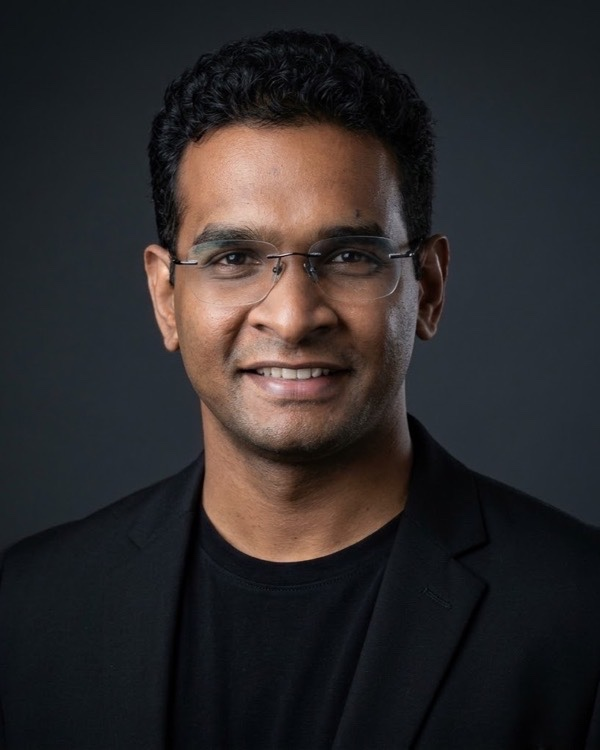
\includegraphics[width=1in,height=1.25in,clip,keepaspectratio]{author.jpg}}]{Bhargava Chary Peddapudi}
received the M.S.\ degree in applied computer science from Northwest Missouri State University, Maryville, MO, USA, in 2015.
He is an independent researcher based in the San Francisco Bay Area, CA, USA.
His research interests include retrieval-augmented generation (RAG) evaluation, metadata-aware vector retrieval, and scaling behavior of approximate nearest-neighbor indexes.
\end{IEEEbiography}

\EOD
\end{document}
